\documentclass{article}
\usepackage[margin=1in]{geometry}
\usepackage[nodisplayskipstretch]{setspace}
\usepackage{amsmath, nccmath, bm}
\usepackage{amssymb}
\usepackage{enumitem}
\usepackage{graphicx}
\usepackage{float}
\usepackage{listings}
\usepackage{hyperref}
\usepackage[svgnames]{xcolor}
\usepackage{indentfirst}
%\usepackage{chngcntr}
%\counterwithin{table}{section}
\graphicspath{
{./images}
{./images/nand}
{./images/nor}}

%\hypersetup{
%    colorlinks=true,
%    linkcolor=black,
%    filecolor=black,      
%    urlcolor=blue
%    }

\newcommand{\zerodisplayskip}{
	\setlength{\abovedisplayskip}{0pt}%
	\setlength{\belowdisplayskip}{0pt}%
	\setlength{\abovedisplayshortskip}{0pt}%
	\setlength{\belowdisplayshortskip}{0pt}%
	\setlength{\mathindent}{0pt}}
	
\definecolor{vgreen}{RGB}{104,180,104}
\definecolor{vblue}{RGB}{49,49,255}
\definecolor{vorange}{RGB}{255,143,102}

\lstdefinestyle{verilog-style}
{
    language=Verilog,
    basicstyle=\small\ttfamily,
    keywordstyle=\color{vblue},
    identifierstyle=\color{black},
    commentstyle=\color{vgreen},
    numbers=left,
    numberstyle=\tiny\color{black},
    numbersep=10pt,
    tabsize=8,
    moredelim=*[s][\colorIndex]{[}{]},
    literate=*{:}{:}1
}

\lstset{style={verilog-style},showstringspaces=false}

\lstdefinestyle{nocoloring}{
    keywordstyle=\color{black},
    commentstyle=\color{black},
    stringstyle=\color{black}
}

\makeatletter
\newcommand*\@lbracket{[}
\newcommand*\@rbracket{]}
\newcommand*\@colon{:}
\newcommand*\colorIndex{%
    \edef\@temp{\the\lst@token}%
    \ifx\@temp\@lbracket \color{black}%
    \else\ifx\@temp\@rbracket \color{black}%
    \else\ifx\@temp\@colon \color{black}%
    \else \color{vorange}%
    \fi\fi\fi
}
\makeatother

\newcommand{\code}[1]{%
	\colorbox{Gainsboro}{\texttt{#1}}%
}

\title{Lab 2}
\author{Owen Sowatzke}
\date{March 31, 2025}

\begin{document}

	% \offinterlineskip
	% \setlength{\lineskip}{12pt}
	% \zerodisplayskip
	\maketitle
	
	\section{Introduction}
	
	In this lab, we learn how to create transistor-level layouts of NAND and NOR gates using MAGIC. After creating our layouts, we verify them using DRC (design rule checks). Then, we extract SPICE netlists for simulation. Finally, we simulate these netlists with ngspice and compare our results to schematic simulations. 
	
	\section{NAND Gate}
	
	\subsection{Layout}
	
	In this section, we review our NAND gate layout, which is displayed in Figure \ref{fig::nand_layout}. The NAND gate is composed of two NMOS transistors in series and two PMOS transistors in parallel. The NMOS transistors lie along the n-diffusion region and the PMOS transistor lie along the p-diffusion regions. The n-diffusion region is placed in the p-type body, and the p-diffusion region is placed in an n-well. Polysilicon is used for the transistor gates. The layout also includes metal1 wires for ground and VDD. The ground wire is connected to the source of the first NMOS transistor with local interconnect (li) material, and the VDD wire is connected to the source of both PMOS transistors with li material. The drain of the last NMOS transistor is connected to the drain of both PMOS transistors with li material to form the gate output. Metal1 contacts are placed on the gate I/O to allow for longer-distance routing. Depending on the distance that the I/O must be routed, li material may be sufficient for the connections. To prevent latchup, the ground wire is also connected to p-substrate diffusion with a substrate tap, and the VDD wire is connected to n-substrate diffusion with a well tap.
	
	\begin{figure}[H]
		\centerline{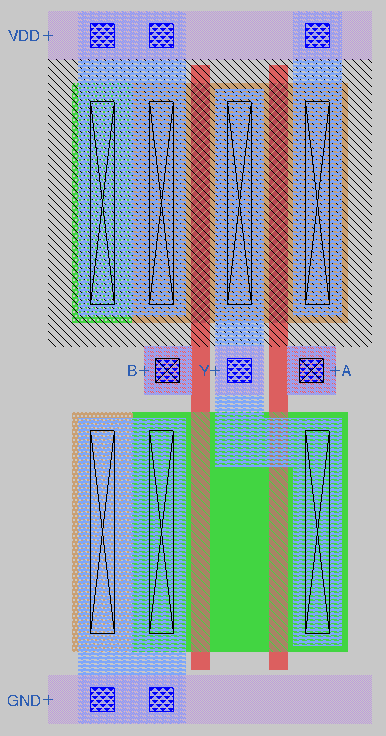
\includegraphics[width=0.3\textwidth]{nand_layout.png}}
		\caption{NAND Gate Layout}
		\label{fig::nand_layout}
	\end{figure}

	Most of the transistor properties are defined by the size of the NMOS and PMOS transistor channels, whose dimensions are shown in Figures \ref{fig::nand_nmos_channel_sizing} and \ref{fig::nand_pmos_channel_sizing}. Note that we have designed the transistors with the minimum channel length for the sky130A technology (150 nm). The channel widths have been chosen to match the delay of an inverter, with $1 {\mu}m$ NMOS channel widths and $2 {\mu}m$ PMOS channel widths. With respect to the inverter, the NAND gate NMOS channel widths have been doubled to $2 {\mu}m$ to maintain the same equivalent resistance. The NAND gate PMOS channel widths are kept the same to maintain the same equivalent resistance for the slowest case (when only when transistor is on).
	
	\begin{figure}[H]
		\centerline{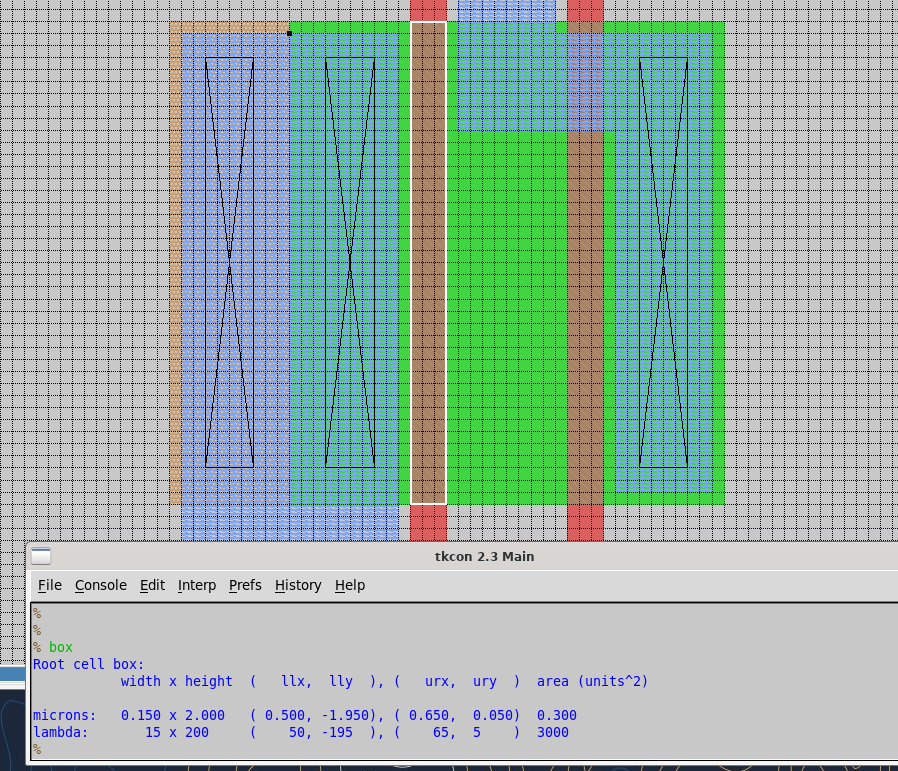
\includegraphics[width=0.5\textwidth]{nand_nmos_channel_sizing.png}}
		\caption{Checking NMOS Channel Size}
		\label{fig::nand_nmos_channel_sizing}
	\end{figure}
	
	\begin{figure}[H]
		\centerline{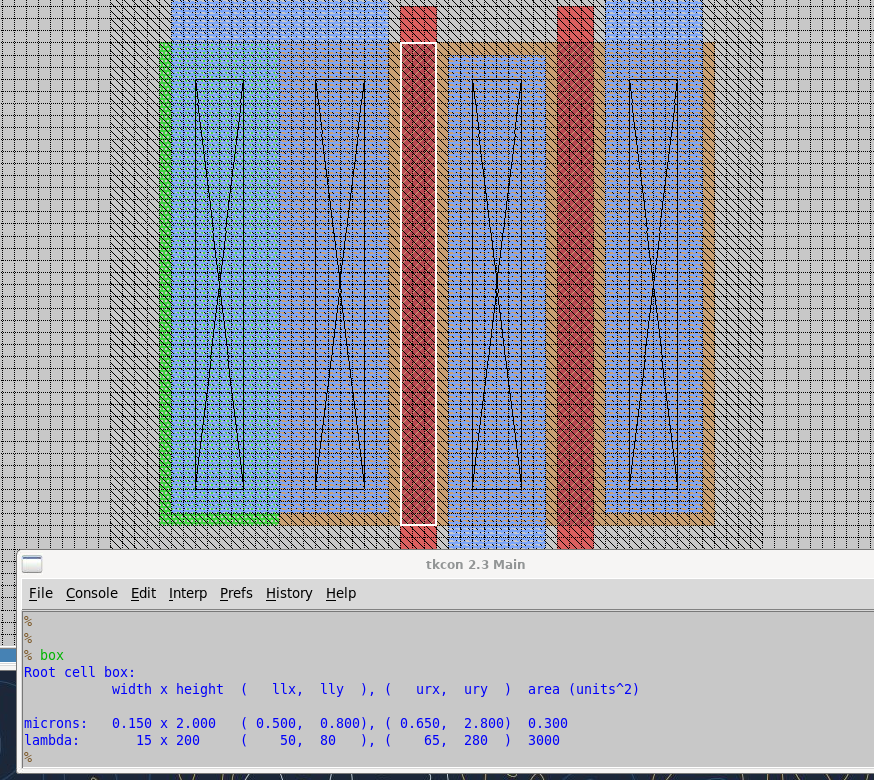
\includegraphics[width=0.5\textwidth]{nand_pmos_channel_sizing.png}}
		\caption{Checking PMOS Channel Size}
		\label{fig::nand_pmos_channel_sizing}
	\end{figure}
	
	For our layout to be valid, it must pass design rule checks (DRC). In Figures \ref{fig::nand_drc_errors_terminal} and \ref{fig::nand_drc_errors_drcmgr}, we confirm that our design meets DRC in two different ways. First, in Figure \ref{fig::nand_drc_errors_terminal}, we use terminal commands to perform a DRC. The \texttt{select} command, selects the entire design, and the \texttt{drc count} and \texttt{drc why} commands return the count and reason for DRC errors respectively. Examining the command outputs, we see that there are no DRC errors. Next, in Figure \ref{fig::nand_drc_errors_drcmgr}, we use the drcmgr to check for DRC errors. Examining the drcmgr output, we see that there are no DRC errors. The primary GUI toolbar also displays a DRC count of 0, which further confirms the validity of our layout.
	
	\begin{figure}[H]
		\centerline{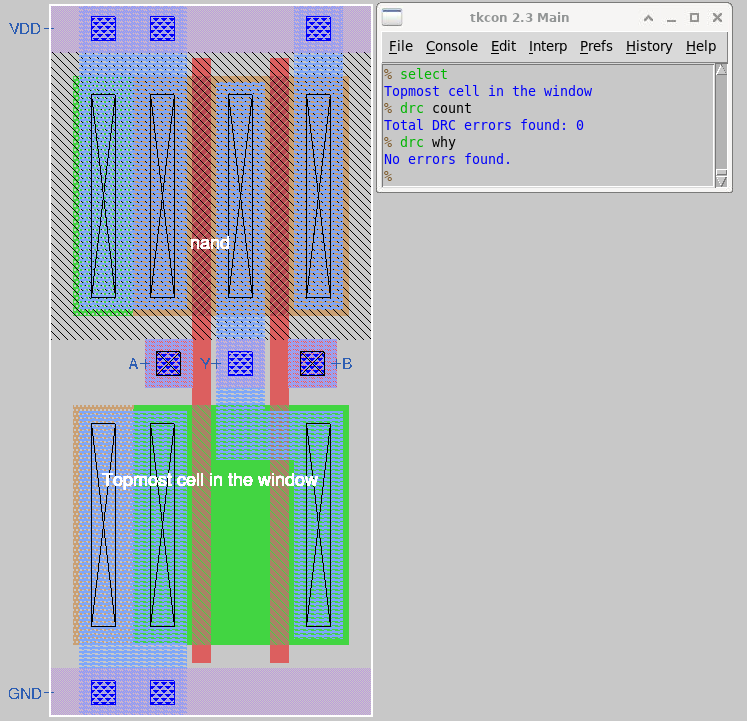
\includegraphics[width=0.5\textwidth]{nand_drc_errors_terminal.png}}
		\caption{Checking DRC Errors from Terminal}
		\label{fig::nand_drc_errors_terminal}
	\end{figure}
	
	\begin{figure}[H]
		\centerline{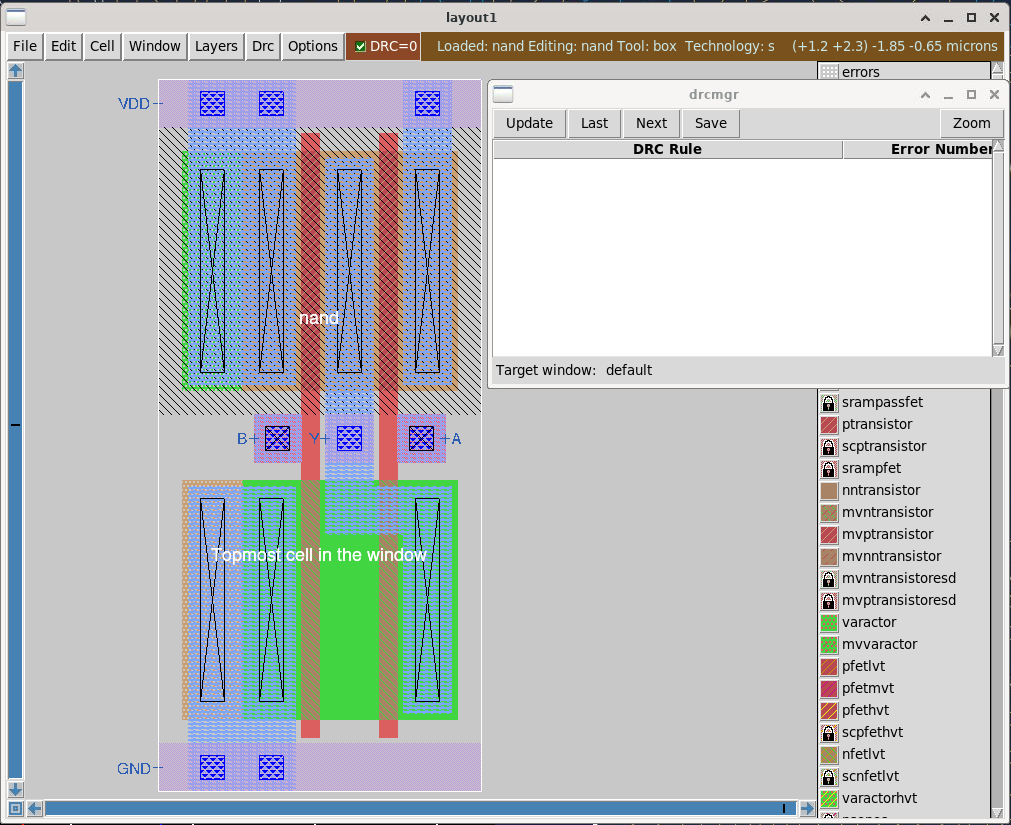
\includegraphics[width=0.5\textwidth]{nand_drc_errors_drcmgr.png}}
		\caption{Checking DRC Errors with drcmgr}
		\label{fig::nand_drc_errors_drcmgr}
	\end{figure}
	
	\subsection{Netlist}
	
	In this section, we generate a netlist from our NAND gate layout. To do so, we specifically follow the commands listed in Figure \ref{fig::nand_netlist_creation}. Note that in addition to the commands provided in the lab description we also run the \texttt{ext2spice} command with the \texttt{lvs} option. This option configures the \texttt{ext2spice} settings for LVS (layout vs schematic simulations) \cite{a2021_magic83}.
	
	\begin{figure}[H]
		\centerline{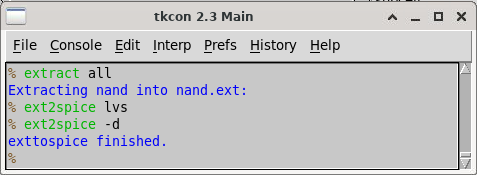
\includegraphics[width=0.3\textwidth]{nand_netlist_creation.png}}
		\caption{SPICE Netlist Extraction}
		\label{fig::nand_netlist_creation}
	\end{figure}
	
	\begin{figure}[H]
		\lstinputlisting[style=nocoloring,frame=single]{./src/nand.spice}
		\caption{Extracted SPICE Netlist for NAND Gate}
		\label{fig::nand_netlist}
	\end{figure}
	
	\subsection{Schematic Simulation}
	
	\begin{figure}[H]
		\centerline{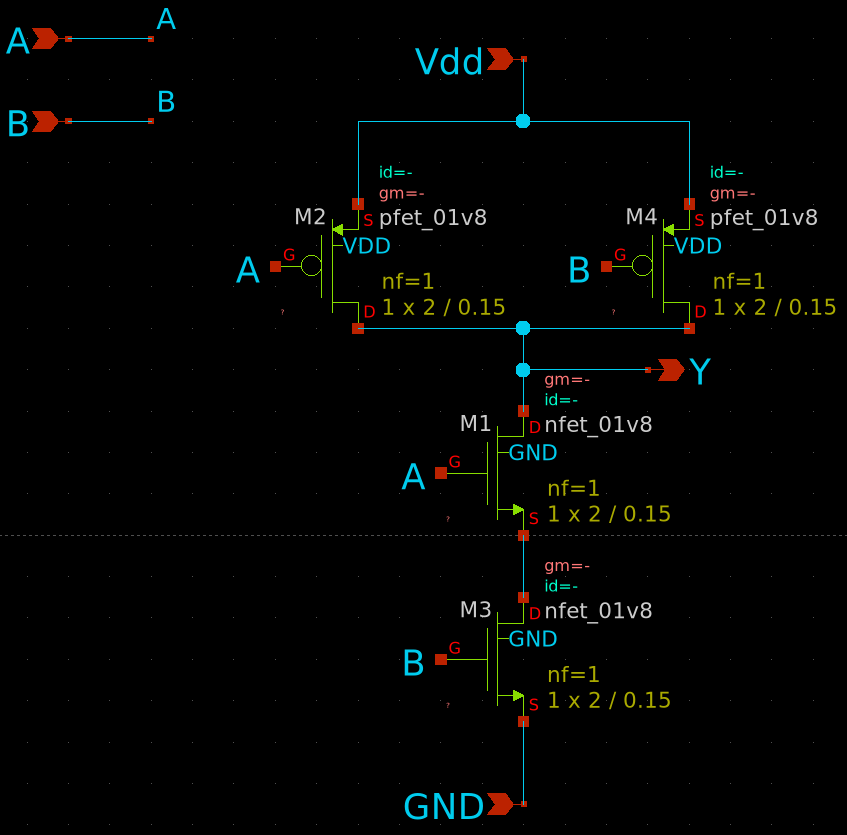
\includegraphics[width=0.5\textwidth]{nand_schematic.png}}
		\caption{NAND Schematic}
		\label{fig::nand_schematic}
	\end{figure}
	
	\begin{figure}[H]
		\centerline{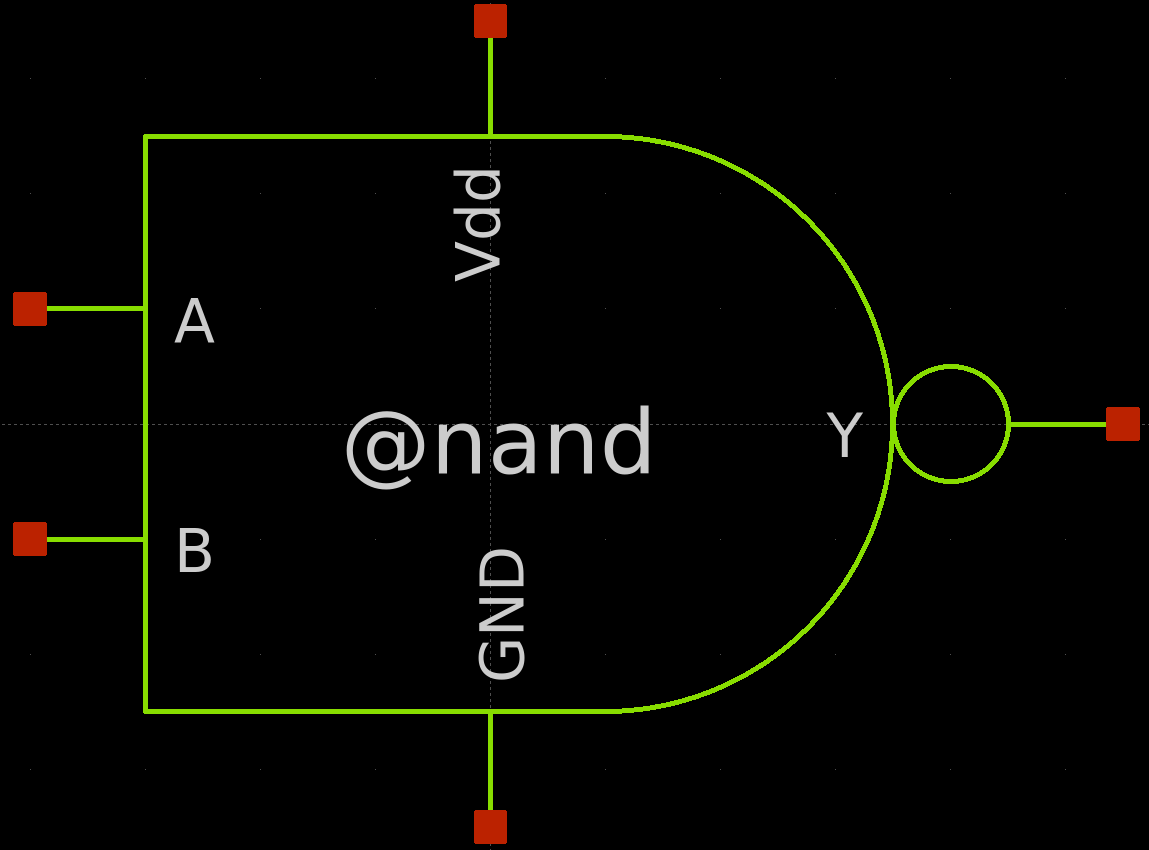
\includegraphics[width=0.3\textwidth]{nand_symbol.png}}
		\caption{NAND Schematic Symbol}
		\label{fig::nand_symbol}
	\end{figure}
	
	\subsection{Simulation Results}
	
	\subsubsection{VTC}
	\begin{figure}[H]
		\lstinputlisting[style=nocoloring,frame=single,basicstyle=\fontsize{7}{7}\selectfont\ttfamily]{./src/nand_vtc.spice}
		\caption{SPICE Test Circuit to Extract VTC from Netlist}
		\label{fig::nand_vtc_test_circuit}
	\end{figure}
	
	\begin{figure}[H]
		\centerline{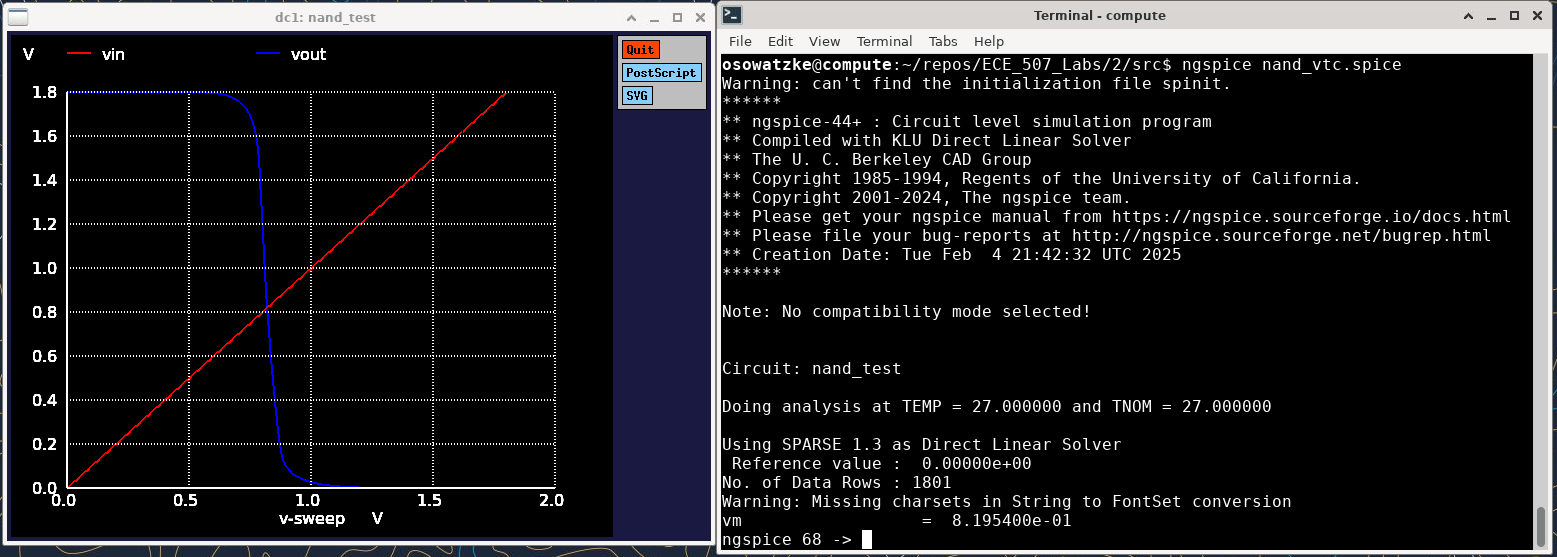
\includegraphics[width=0.8\textwidth]{nand_vtc.png}}
		\caption{VTC from Netlist Simulation}
		\label{fig::nand_vtc}
	\end{figure}
	
	\begin{figure}[H]
		\centerline{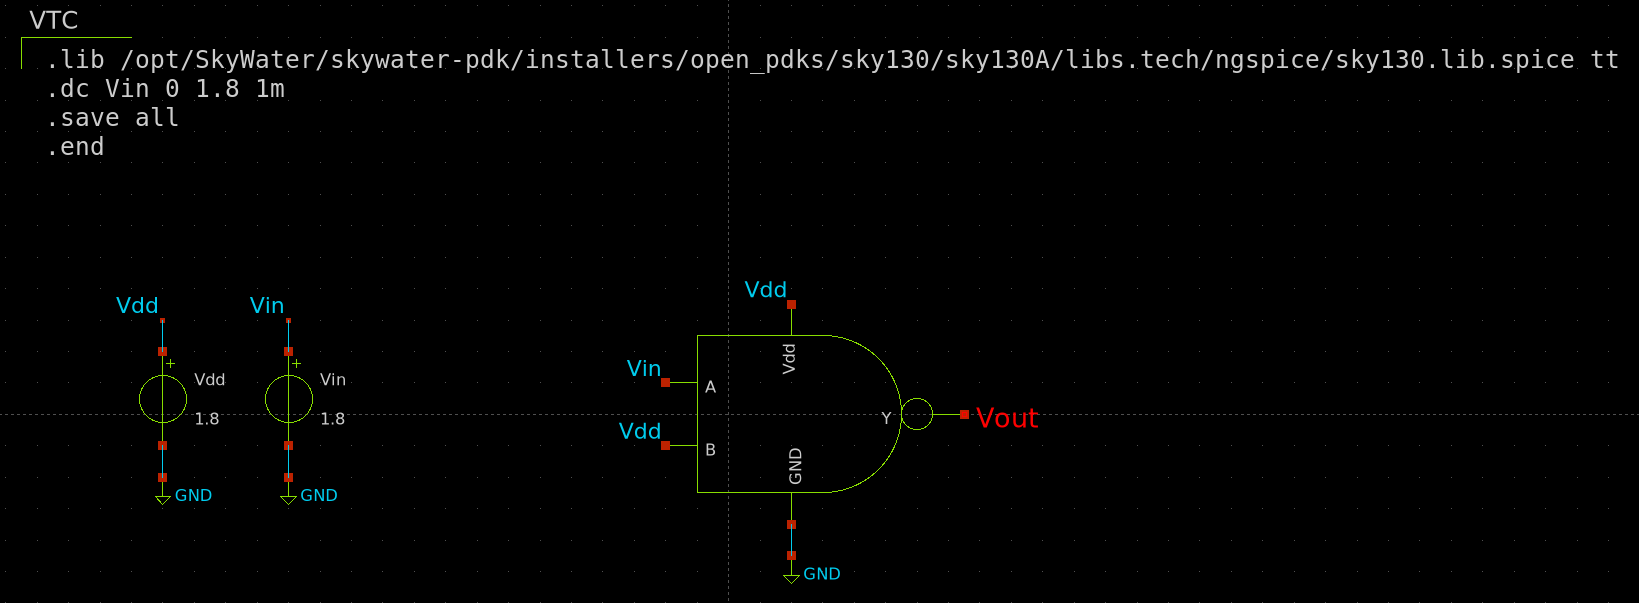
\includegraphics[width=0.8\textwidth]{nand_vtc_test_circuit.png}}
		\caption{Schematic Test Circuit to Collect NAND Gate VTC}
		\label{fig::nand_vtc_schem_test_circuit}
	\end{figure}
	
	\begin{figure}[H]
		\centerline{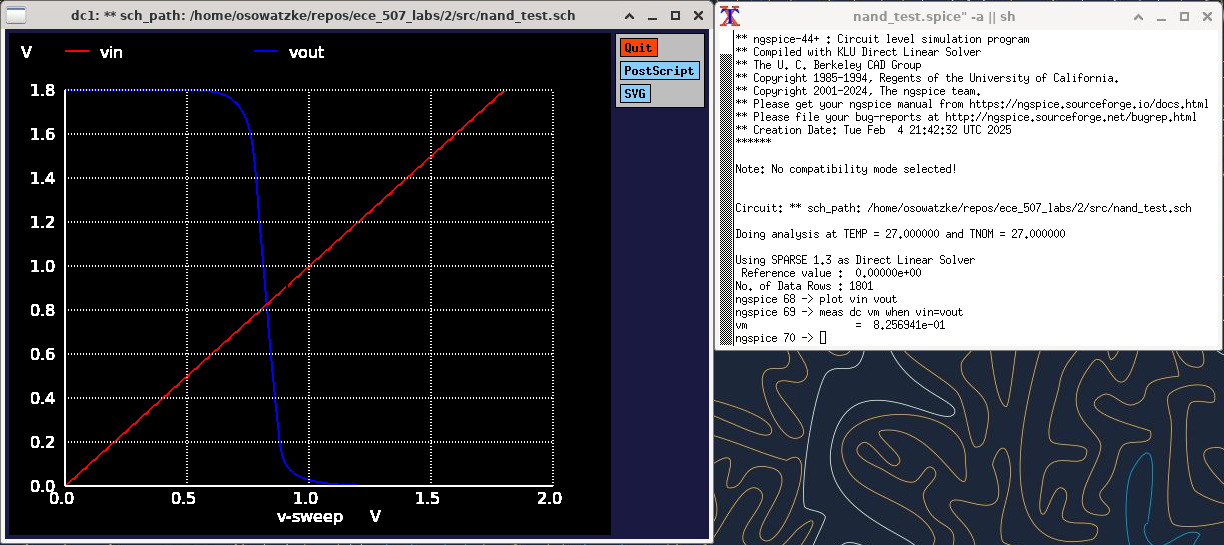
\includegraphics[width=0.8\textwidth]{nand_vtc_schem.png}}
		\caption{VTC from Schematic Simulation}
		\label{fig::nand_vtc_schem}
	\end{figure}
	
	\begin{table}[H]
	\begin{center}
	\caption{VTC Netlist Results}
	\label{table::vtc_netlist}
	\begin{tabular}{| c | c | c |}
		\hline
		\texttt{a} & \texttt{b} & \texttt{Vm}\\
		\hline	
		$0 \rightarrow 1$ & $1$ & $0.8257\ \text{V}$\\
		\hline	
		$1$ & $0 \rightarrow 1$ & $0.8195\ \text{V}$\\
		\hline	
		$0 \rightarrow 1$ & $0 \rightarrow 1$ & $0.9108\ \text{V}$\\
		\hline
	\end{tabular}
	\end{center}
	\end{table}
	
	\begin{table}[H]
	\begin{center}
	\caption{VTC Schematic Results}
	\label{table::vtc_schematic}
	\begin{tabular}{| c | c | c |}
		\hline
		\texttt{a} & \texttt{b} & \texttt{Vm}\\
		\hline	
		$0 \rightarrow 1$ & $1$ & $0.8257\ \text{V}$\\
		\hline	
		$1$ & $0 \rightarrow 1$ & $0.8195\ \text{V}$\\
		\hline	
		$0 \rightarrow 1$ & $0 \rightarrow 1$ & $0.9108\ \text{V}$\\
		\hline
	\end{tabular}
	\end{center}
	\end{table}
	
	\subsubsection{Noise Analysis}
	\begin{figure}[H]
		\lstinputlisting[style=nocoloring,frame=single,basicstyle=\fontsize{7}{7}\selectfont\ttfamily]{./src/nand_noise_analysis.spice}
		\caption{SPICE Test Circuit to Perform Noise Analysis on Netlist}
		\label{fig::nand_noise_analysis_test_circuit}
	\end{figure}
	
	\begin{figure}[H]
		\centerline{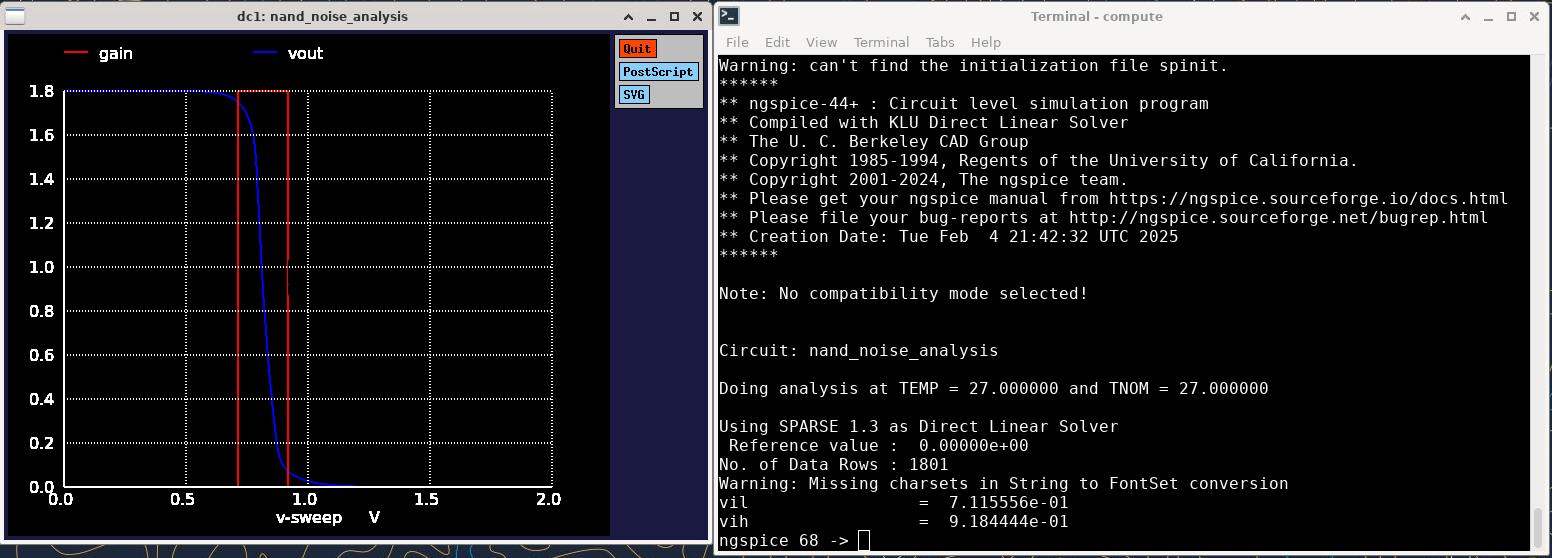
\includegraphics[width=0.8\textwidth]{nand_noise_analysis.png}}
		\caption{Noise Analysis Results from Netlist Simulation}
		\label{fig::nand_noise_analysis}
	\end{figure}
	
	\begin{figure}[H]
		\centerline{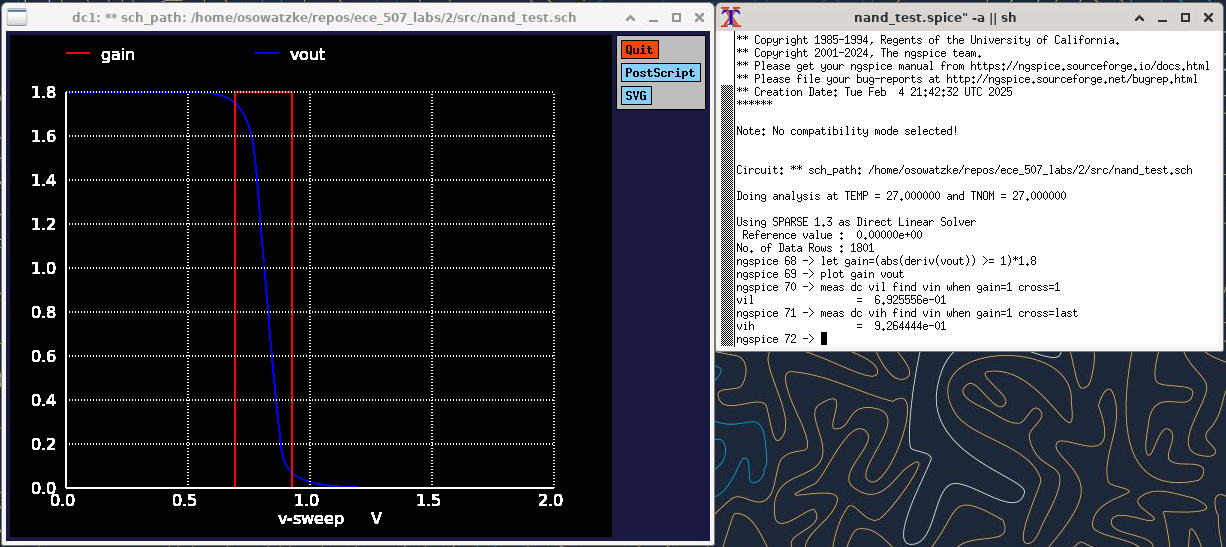
\includegraphics[width=0.8\textwidth]{nand_noise_analysis_schem.png}}
		\caption{Noise Analysis Results from Schematic Simulation}
		\label{fig::nand_noise_analysis_schem}
	\end{figure}
	
	\begin{table}[H]
	\begin{center}
	\caption{Noise Margins from Netlist Simulation}
	\label{table::nand_gate_noise_analysis}
	\begin{tabular}{| c | c | c | c | c | c |}
		\hline
		\texttt{a} & \texttt{b} & \texttt{Vih} & \texttt{Vil} & \texttt{Nmh} & \texttt{Nml} \\
		\hline	
		$0 \rightarrow 1$ & $1$ & $0.9264 \text{V}$ & $0.6926 \text{V}$ & $0.8736 \text{V}$ & $0.6926 \text{V}$\\
		\hline	
		$1$ & $0 \rightarrow 1$ & $0.9184 \text{V}$ & $0.7116 \text{V}$ & $0.8816 \text{V}$ & $0.7116 \text{V}$\\
		\hline	
		$0 \rightarrow 1$ & $0 \rightarrow 1$ & $1.0224 \text{V}$ & $0.8046 \text{V}$ & $0.7776 \text{V}$ & $0.7776 \text{V}$\\
		\hline
	\end{tabular}
	\end{center}
	\end{table}
	
	\begin{table}[H]
	\begin{center}
	\caption{Noise Margins from Schematic Simulation}
	\label{table::nand_gate_noise_analysis_schem}
	\begin{tabular}{| c | c | c | c | c | c |}
		\hline
		\texttt{a} & \texttt{b} & \texttt{Vih} & \texttt{Vil} & \texttt{Nmh} & \texttt{Nml} \\
		\hline	
		$0 \rightarrow 1$ & $1$ & $0.9264 \text{V}$ & $0.6926 \text{V}$ & $0.8736 \text{V}$ & $0.6926 \text{V}$\\
		\hline	
		$1$ & $0 \rightarrow 1$ & $0.9184 \text{V}$ & $0.7116 \text{V}$ & $0.8816 \text{V}$ & $0.7116 \text{V}$\\
		\hline	
		$0 \rightarrow 1$ & $0 \rightarrow 1$ & $1.0224 \text{V}$ & $0.8046 \text{V}$ & $0.7776 \text{V}$ & $0.7776 \text{V}$\\
		\hline
	\end{tabular}
	\end{center}
	\end{table}
	
	\subsubsection{Delay Analysis}
	\begin{figure}[H]
		\lstinputlisting[style=nocoloring,frame=single,basicstyle=\fontsize{7}{7}\selectfont\ttfamily]{./src/nand_delay_analysis.spice}
		\caption{SPICE Test Circuit to Perform Delay Analysis on Netlist}
		\label{fig::nand_delay_analysis_test_circuit}
	\end{figure}
	
	\begin{figure}[H]
		\centerline{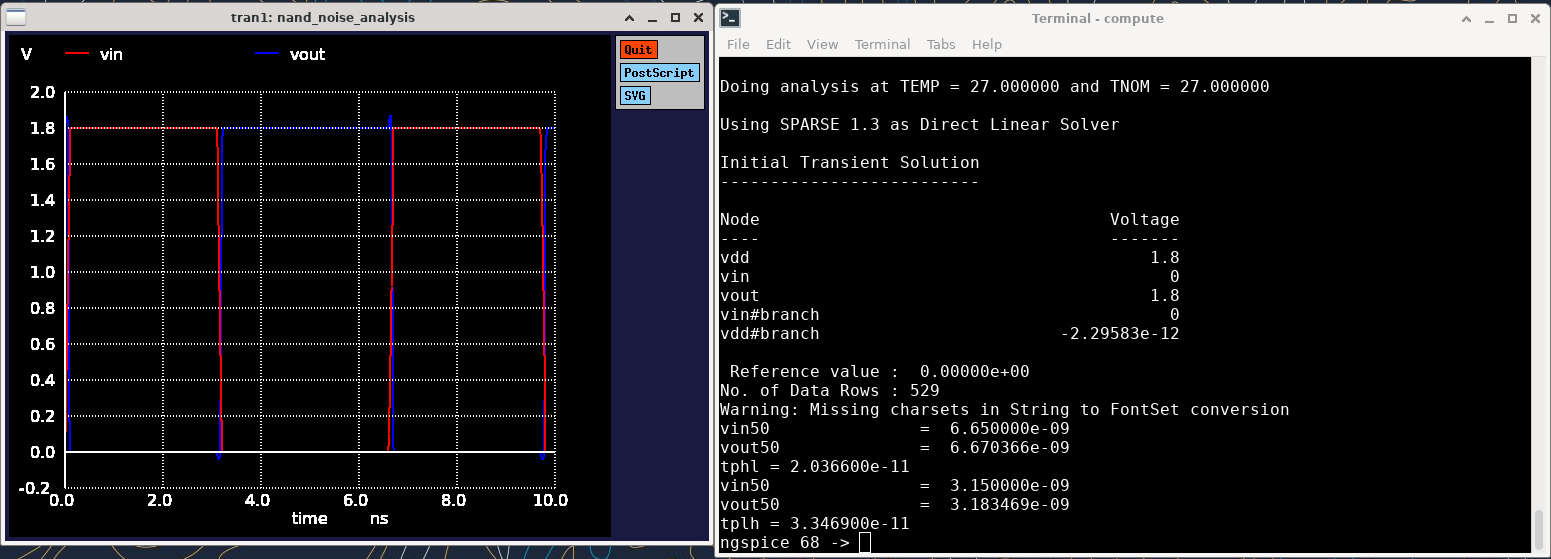
\includegraphics[width=0.8\textwidth]{nand_delay_analysis.png}}
		\caption{Delay Analysis Results from Netlist Simulation}
		\label{fig::nand_delay_analysis}
	\end{figure}
	
	\begin{figure}[H]
		\centerline{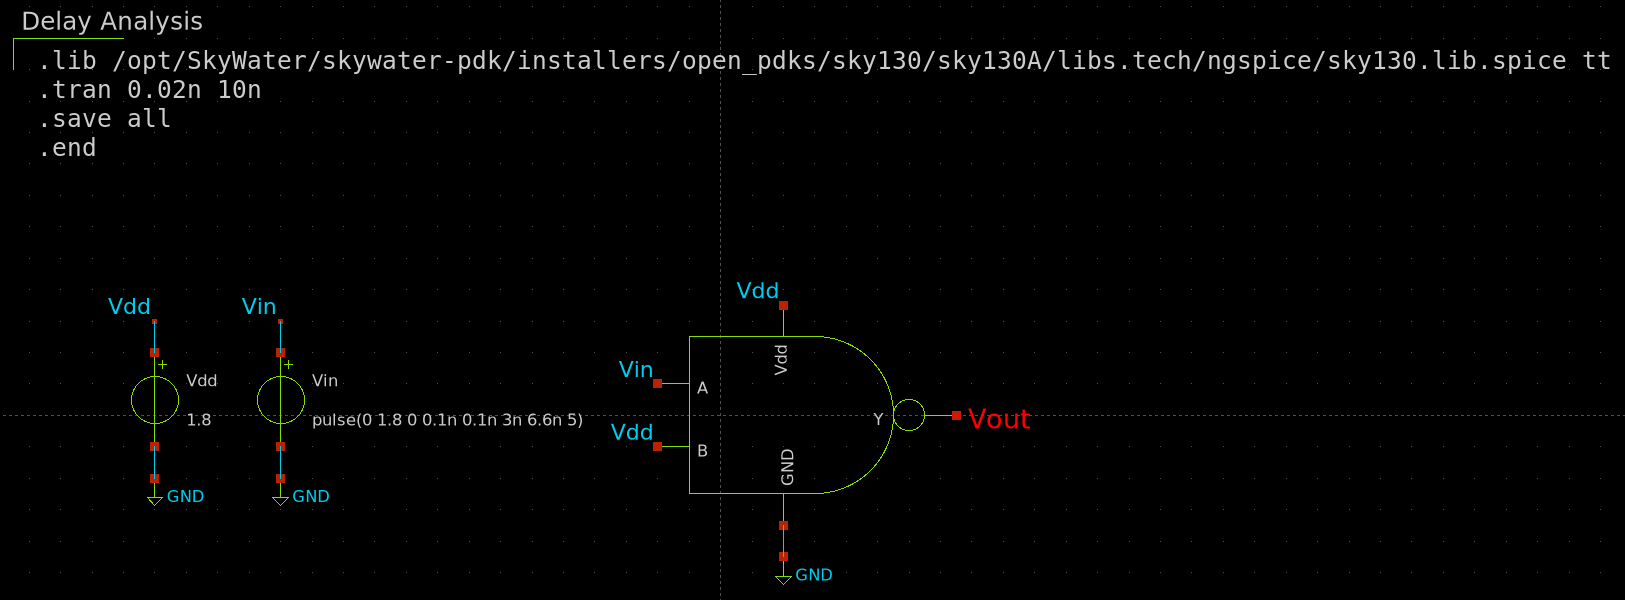
\includegraphics[width=0.8\textwidth]{nand_delay_analysis_test_circuit.png}}
		\caption{Schematic Test Circuit for NAND Gate Delay Analysis}
		\label{fig::nand_delay_analysis_test_circuit_schem}
	\end{figure}
	
	\begin{figure}[H]
		\centerline{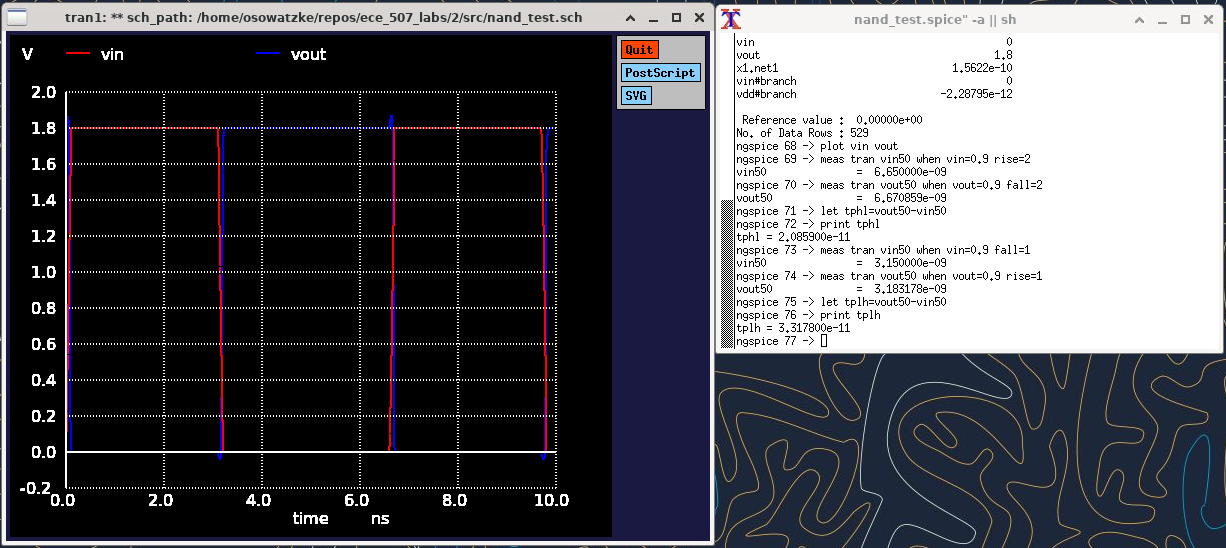
\includegraphics[width=0.8\textwidth]{nand_delay_analysis_schem.png}}
		\caption{Delay Analysis Results from Schematic Simulation}
		\label{fig::nand_delay_analysis_schem}
	\end{figure}
	
	\begin{table}[H]
	\begin{center}
	\caption{Delay from Netlist Simulation}
	\label{table::nand_gate_delay_analysis}
	\begin{tabular}{| c | c | c || c | c | c |}
		\hline
		\texttt{a} & \texttt{b} & \texttt{tphl} & \texttt{a} & \texttt{b} & \texttt{tplh} \\
		\hline	
		$0 \rightarrow 1$ & $1$ & $20.336\ \text{ps}$ & $1 \rightarrow 0$ & $1$ & $33.469\ \text{ps}$\\
		\hline	
		$1$ & $0 \rightarrow 1$ & $27.766\ \text{ps}$ & $1$ & $1 \rightarrow 0$ & $47.659\ \text{ps}$\\
		\hline	
		$0 \rightarrow 1$ & $0 \rightarrow 1$ & $29.263\ \text{ps}$ & $1 \rightarrow 0$ & $1 \rightarrow 0$ & $26.400\ \text{ps}$\\
		\hline
	\end{tabular}
	\end{center}
	\end{table}
	
	\begin{table}[H]
	\begin{center}
	\caption{Delay from Schematic Simulation}
	\label{table::nand_gate_delay_analysis_schem}
	\begin{tabular}{| c | c | c || c | c | c |}
		\hline
		\texttt{a} & \texttt{b} & \texttt{tphl} & \texttt{a} & \texttt{b} & \texttt{tplh} \\
		\hline	
		$0 \rightarrow 1$ & $1$ & $20.859\ \text{ps}$ & $1 \rightarrow 0$ & $1$ & $33.178\ \text{ps}$\\
		\hline	
		$1$ & $0 \rightarrow 1$ & $28.416\ \text{ps}$ & $1$ & $1 \rightarrow 0$ & $48.137\ \text{ps}$\\
		\hline	
		$0 \rightarrow 1$ & $0 \rightarrow 1$ & $29.297\ \text{ps}$ & $1 \rightarrow 0$ & $1 \rightarrow 0$ & $26.097\ \text{ps}$\\
		\hline
	\end{tabular}
	\end{center}
	\end{table}
	
	\subsubsection{Power Analysis}
	\begin{figure}[H]
		\lstinputlisting[style=nocoloring,frame=single,basicstyle=\fontsize{7}{7}\selectfont\ttfamily]{./src/nand_power_analysis.spice}
		\caption{SPICE Test Circuit to Perform Power Analysis on Netlist}
		\label{fig::nand_power_analysis_test_circuit}
	\end{figure}
	
	\begin{figure}[H]
		\centerline{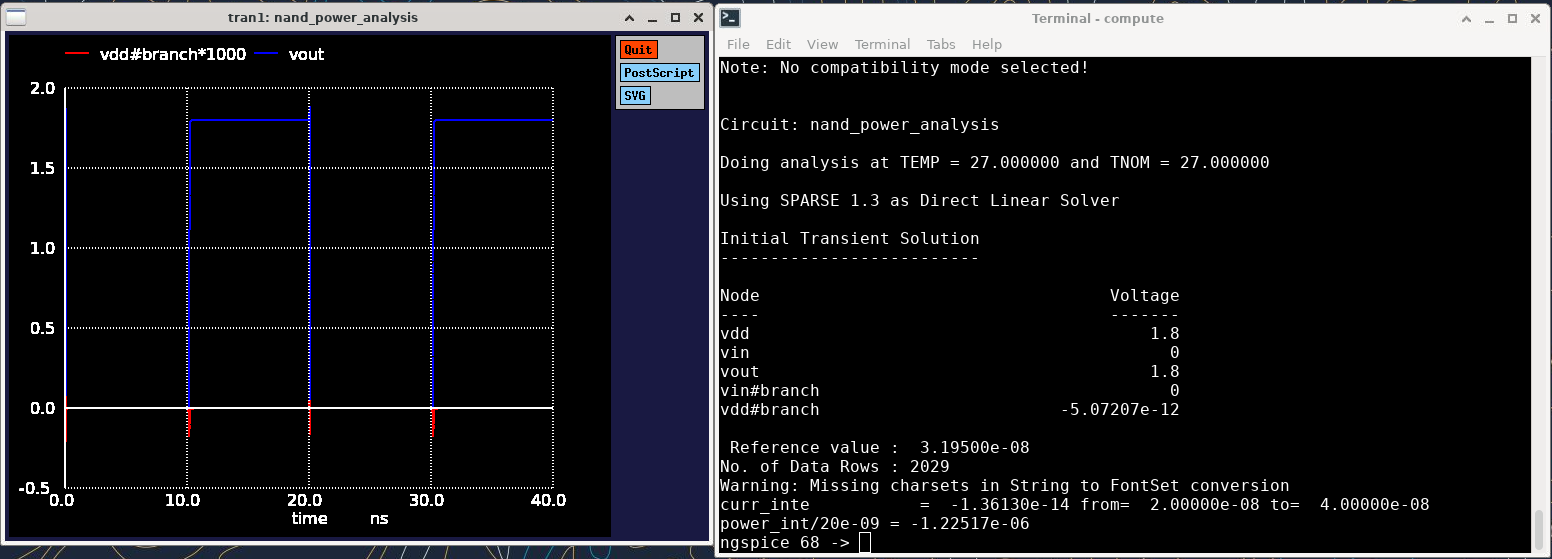
\includegraphics[width=0.8\textwidth]{nand_power_analysis.png}}
		\caption{Power Analysis Results from Netlist Simulation}
		\label{fig::nand_power_analysis}
	\end{figure}
	
	\begin{figure}[H]
		\centerline{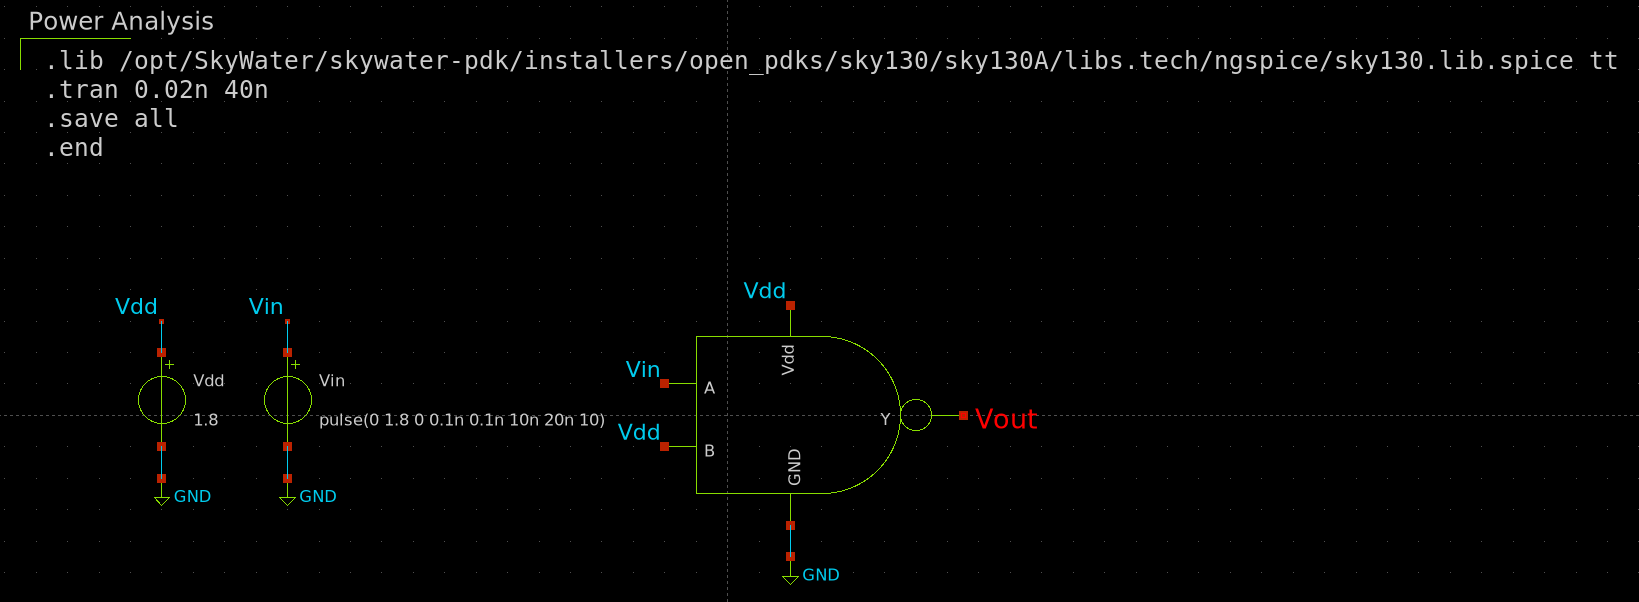
\includegraphics[width=0.8\textwidth]{nand_power_analysis_test_circuit.png}}
		\caption{Schematic Test Circuit for NAND Gate Power Analysis}
		\label{fig::nand_power_analysis_test_circuit_schem}
	\end{figure}
	
	\begin{figure}[H]
		\centerline{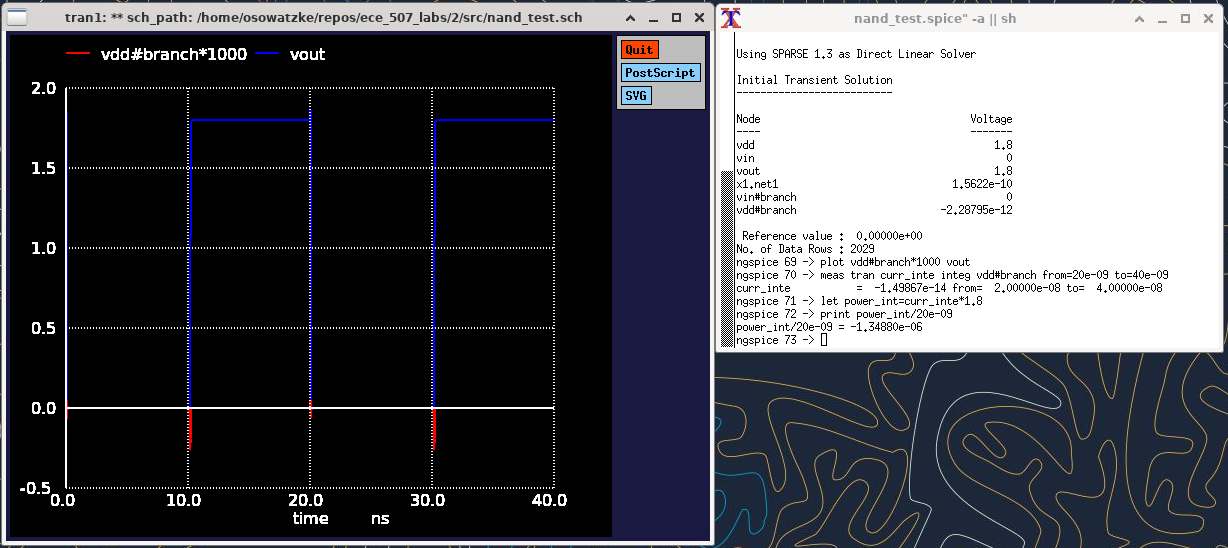
\includegraphics[width=0.8\textwidth]{nand_power_analysis_schem.png}}
		\caption{Power Analysis Results from Schematic Simulation}
		\label{fig::nand_power_analysis_schem}
	\end{figure}
	
	\begin{table}[H]
	\begin{center}
	\caption{Power Consumption from Netlist Simulation}
	\label{table::nand_gate_power_analysis}
	\begin{tabular}{| c | c | c |}
		\hline
		\texttt{a} & \texttt{b} & \texttt{Power}\\
		\hline	
		$0 \rightarrow 1 \rightarrow 0$ & $1$ & $1.34724{\mu}W$ \\
		\hline	
		$1$ & $0 \rightarrow 1 \rightarrow 0$ & $1.85866{\mu}W$ \\
		\hline	
		$0 \rightarrow 1 \rightarrow 0$ & $0 \rightarrow 1 \rightarrow 0$ & $1.44641{\mu}W$\\
		\hline
	\end{tabular}
	\end{center}
	\end{table}
	
	\begin{table}[H]
	\begin{center}
	\caption{Power Consumption from Schematic Simulation}
	\label{table::nand_gate_power_analysis_schem}
	\begin{tabular}{| c | c | c |}
		\hline
		\texttt{a} & \texttt{b} & \texttt{Power}\\
		\hline	
		$0 \rightarrow 1 \rightarrow 0$ & $1$ & $1.34880{\mu}W$ \\
		\hline	
		$1$ & $0 \rightarrow 1 \rightarrow 0$ & $1.88943{\mu}W$ \\
		\hline	
		$0 \rightarrow 1 \rightarrow 0$ & $0 \rightarrow 1 \rightarrow 0$ & $1.44446{\mu}W$\\
		\hline
	\end{tabular}
	\end{center}
	\end{table}
	
	\section{NOR Gates}
	
	\subsection{Layout}
	
	\begin{figure}[H]
		\centerline{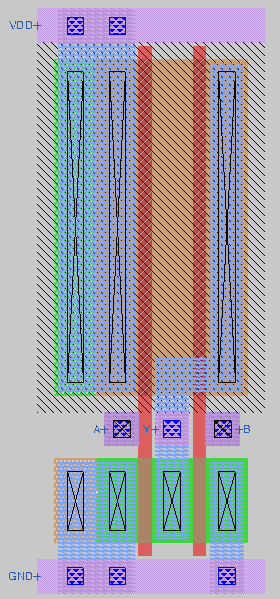
\includegraphics[width=0.3\textwidth]{nor_layout.png}}
		\caption{NOR Gate Layout}
		\label{fig::nor_layout}
	\end{figure}
	
	\begin{figure}[H]
		\centerline{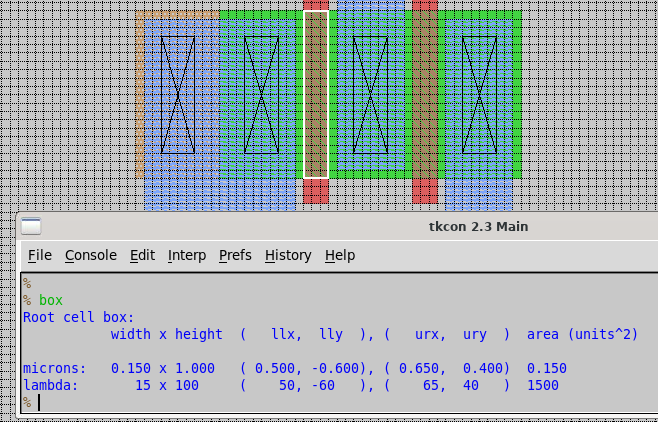
\includegraphics[width=0.5\textwidth]{nor_nmos_channel_sizing.png}}
		\caption{Checking NMOS Channel Size}
		\label{fig::nor_nmos_channel_sizing}
	\end{figure}
	
	\begin{figure}[H]
		\centerline{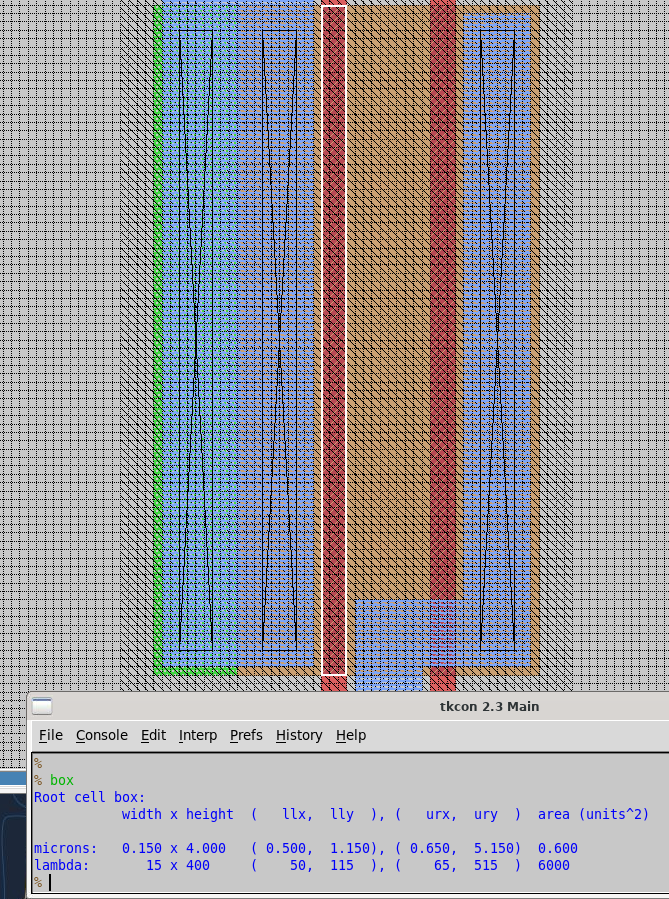
\includegraphics[width=0.5\textwidth]{nor_pmos_channel_sizing.png}}
		\caption{Checking PMOS Channel Size}
		\label{fig::nor_pmos_channel_sizing}
	\end{figure}
	
	\begin{figure}[H]
		\centerline{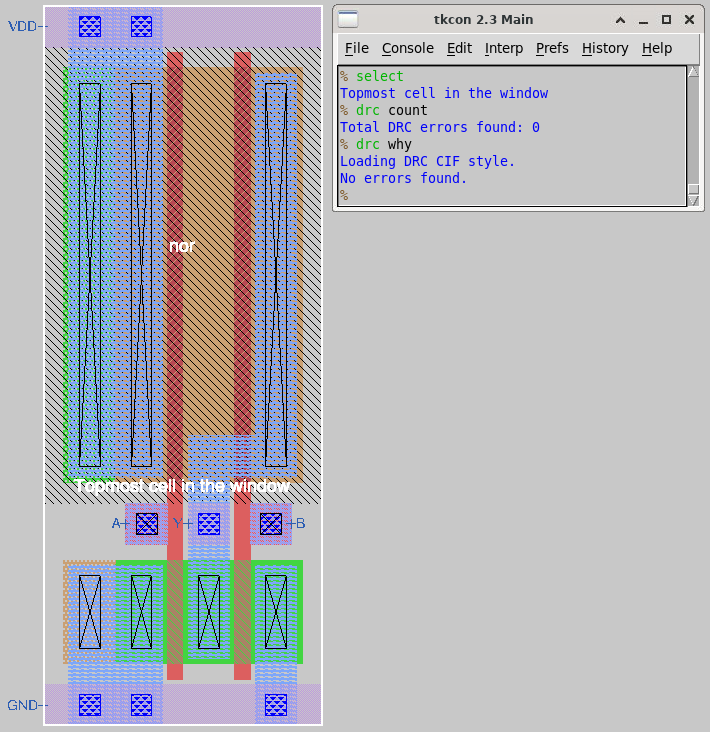
\includegraphics[width=0.5\textwidth]{nor_drc_errors_terminal.png}}
		\caption{Checking DRC Errors from Terminal}
		\label{fig::nor_drc_errors_terminal}
	\end{figure}
	
	\begin{figure}[H]
		\centerline{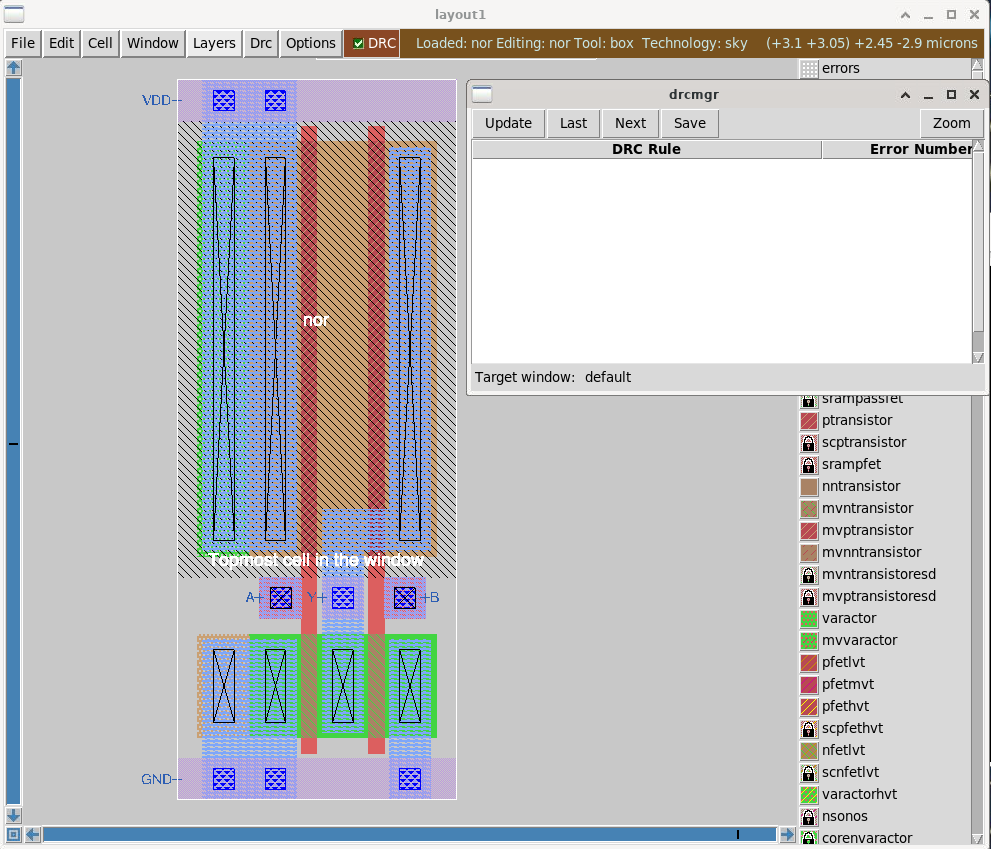
\includegraphics[width=0.5\textwidth]{nor_drc_errors_drcmgr.png}}
		\caption{Checking DRC Errors with drcmgr}
		\label{fig::nor_drc_errors_drcmgr}
	\end{figure}
	
	\subsection{Netlist}
	
	\begin{figure}[H]
		\lstinputlisting[style=nocoloring,frame=single]{./src/nor.spice}
		\caption{Extracted SPICE Netlist for NOR Gate}
		\label{fig::nor_netlist}
	\end{figure}
	
	\subsection{Schematic Simulation}
	
	\begin{figure}[H]
		\centerline{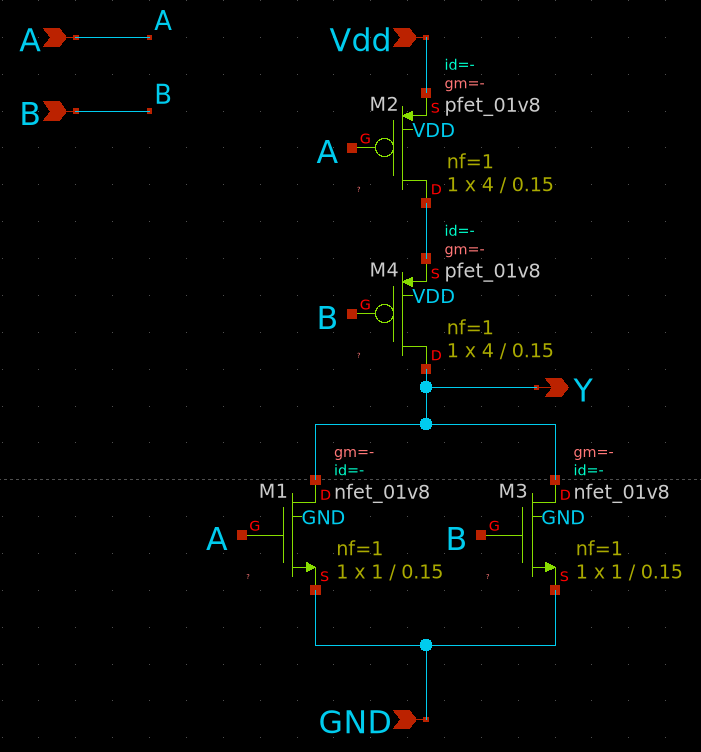
\includegraphics[width=0.5\textwidth]{nor_schematic.png}}
		\caption{NOR Schematic}
		\label{fig::nor_sechematic}
	\end{figure}
	
	\begin{figure}[H]
		\centerline{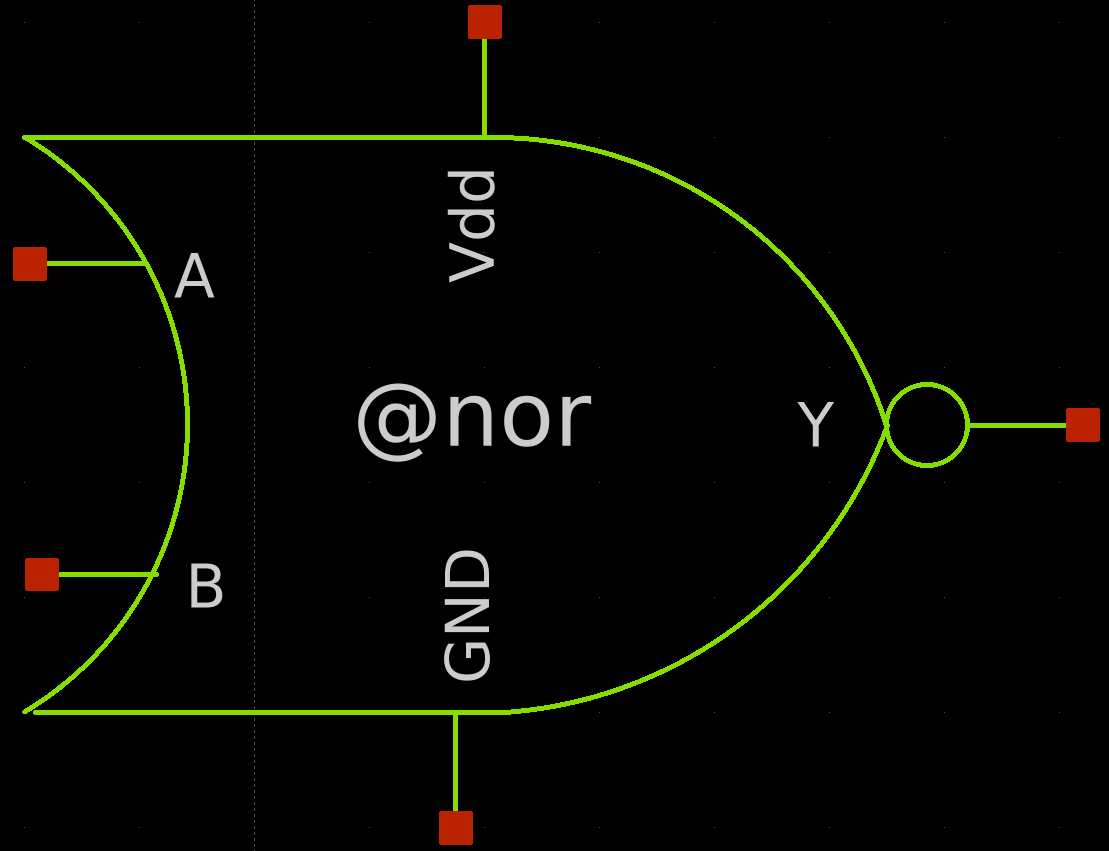
\includegraphics[width=0.3\textwidth]{nor_symbol.png}}
		\caption{NOR Schematic Symbol}
		\label{fig::nor_symbol}
	\end{figure}
	
	\subsection{Simulation Results}
	
	\subsubsection{VTC}
	
	\begin{figure}[H]
		\lstinputlisting[style=nocoloring,frame=single,basicstyle=\fontsize{7}{7}\selectfont\ttfamily]{./src/nor_vtc.spice}
		\caption{SPICE Test Circuit to Extract VTC from Netlist}
		\label{fig::nor_vtc_test_circuit}
	\end{figure}
	
	\begin{figure}[H]
		\centerline{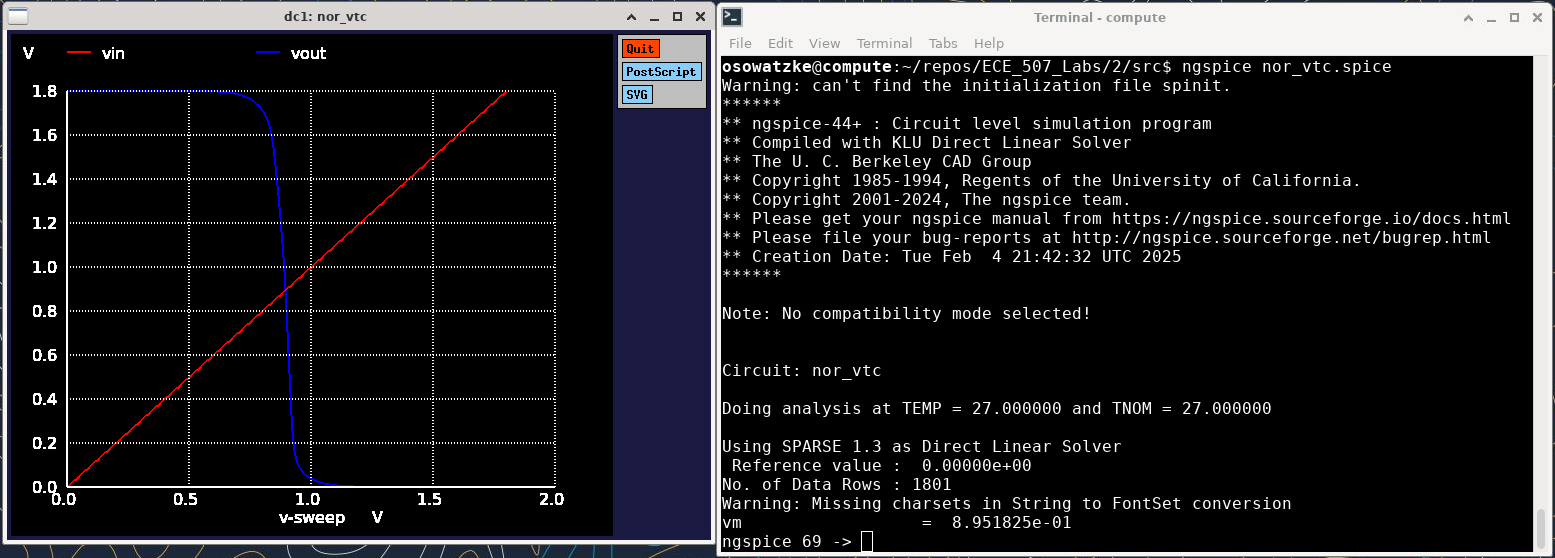
\includegraphics[width=0.8\textwidth]{nor_vtc.png}}
		\caption{VTC from Netlist Simulation}
		\label{fig::nor_vtc}
	\end{figure}
	
	\begin{figure}[H]
		\centerline{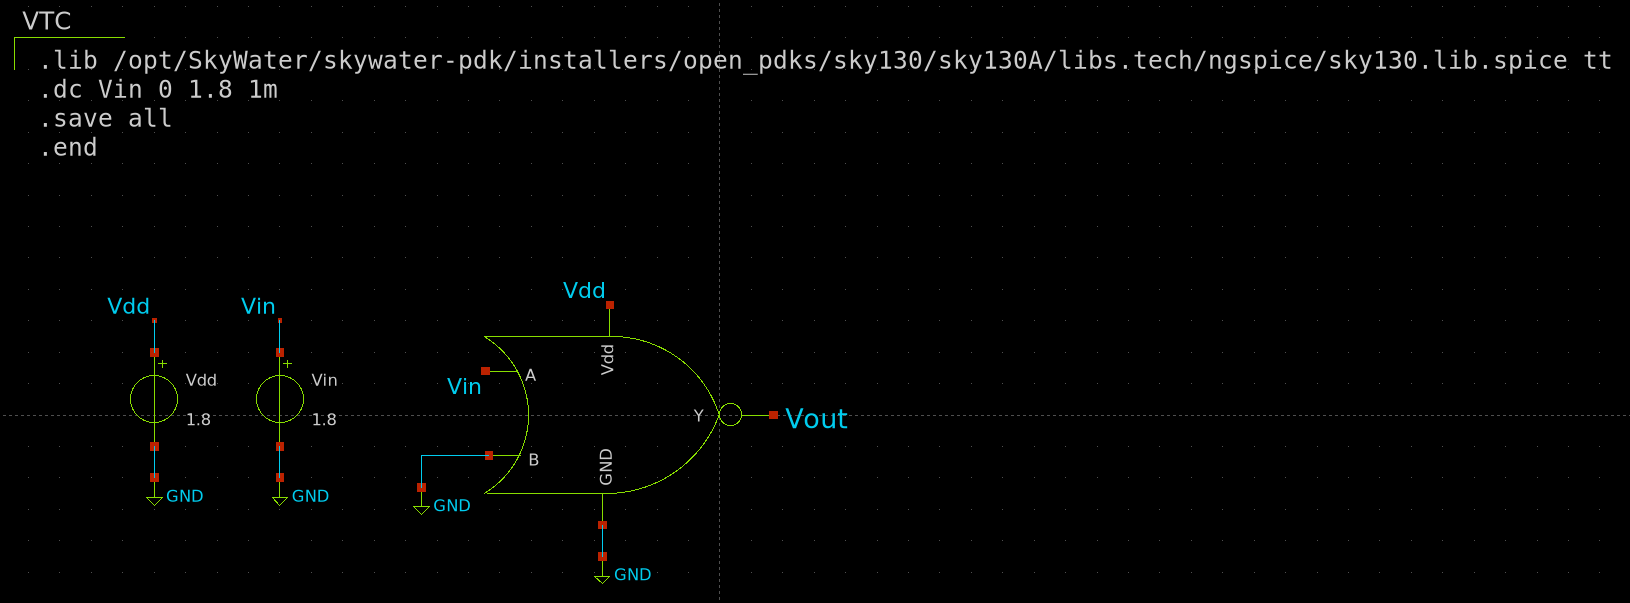
\includegraphics[width=0.8\textwidth]{nor_vtc_test_circuit.png}}
		\caption{Schematic Test Circuit for Collect NOR Gate VTC}
		\label{fig::nor_vtc_schem_test_circuit}
	\end{figure}
	
	\begin{figure}[H]
		\centerline{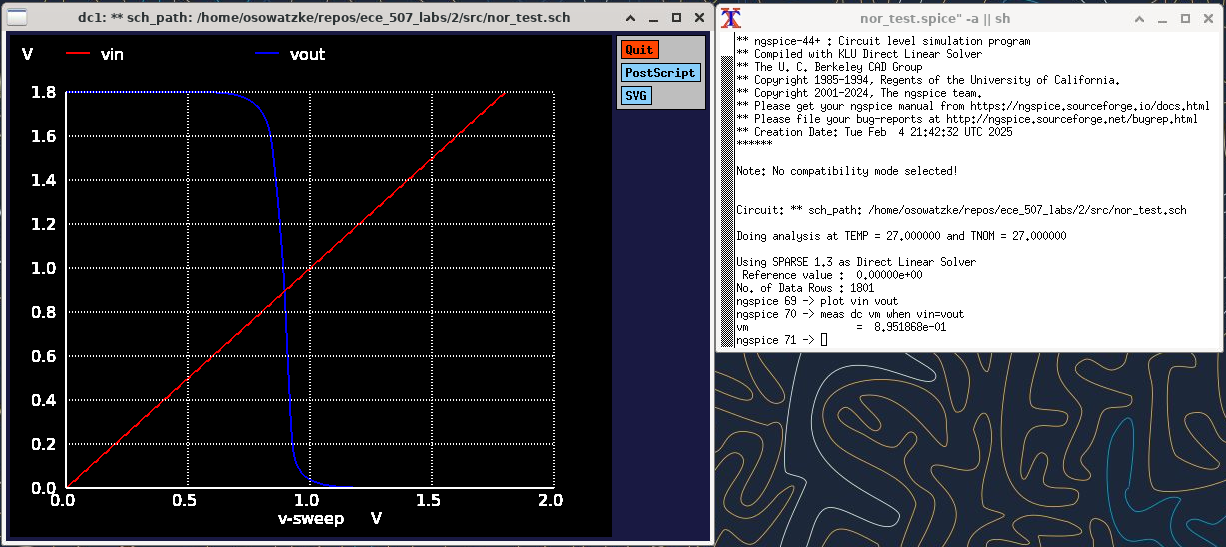
\includegraphics[width=0.8\textwidth]{nor_vtc_schem.png}}
		\caption{VTC from Schematic Simulation}
		\label{fig::nor_vtc_schem}
	\end{figure}
	
	\begin{table}[H]
	\begin{center}
	\caption{VTC Netlist Results}
	\label{table::nor_vtc_netlist}
	\begin{tabular}{| c | c | c |}
		\hline
		\texttt{a} & \texttt{b} & \texttt{Vm}\\
		\hline	
		$0 \rightarrow 1$ & $0$ & $0.8952\ \text{V}$\\
		\hline	
		$0$ & $0 \rightarrow 1$ & $0.8919\ \text{V}$\\
		\hline	
		$0 \rightarrow 1$ & $0 \rightarrow 1$ & $0.8078\ \text{V}$\\
		\hline
	\end{tabular}
	\end{center}
	\end{table}
	
	\begin{table}[H]
	\begin{center}
	\caption{VTC Schematic Results}
	\label{table::nor_vtc_schematic}
	\begin{tabular}{| c | c | c |}
		\hline
		\texttt{a} & \texttt{b} & \texttt{Vm}\\
		\hline	
		$0 \rightarrow 1$ & $0$ & $0.8952\ \text{V}$\\
		\hline	
		$0$ & $0 \rightarrow 1$ & $0.8919\ \text{V}$\\
		\hline	
		$0 \rightarrow 1$ & $0 \rightarrow 1$ & $0.8078\ \text{V}$\\
		\hline
	\end{tabular}
	\end{center}
	\end{table}
	
	\subsubsection{Noise Analysis}
	
	\begin{figure}[H]
		\lstinputlisting[style=nocoloring,frame=single,basicstyle=\fontsize{7}{7}\selectfont\ttfamily]{./src/nor_noise_analysis.spice}
		\caption{SPICE Test Circuit to Perform Noise Analysis on Netlist}
		\label{fig::nor_noise_analysis_test_circuit}
	\end{figure}
	
	\begin{figure}[H]
		\centerline{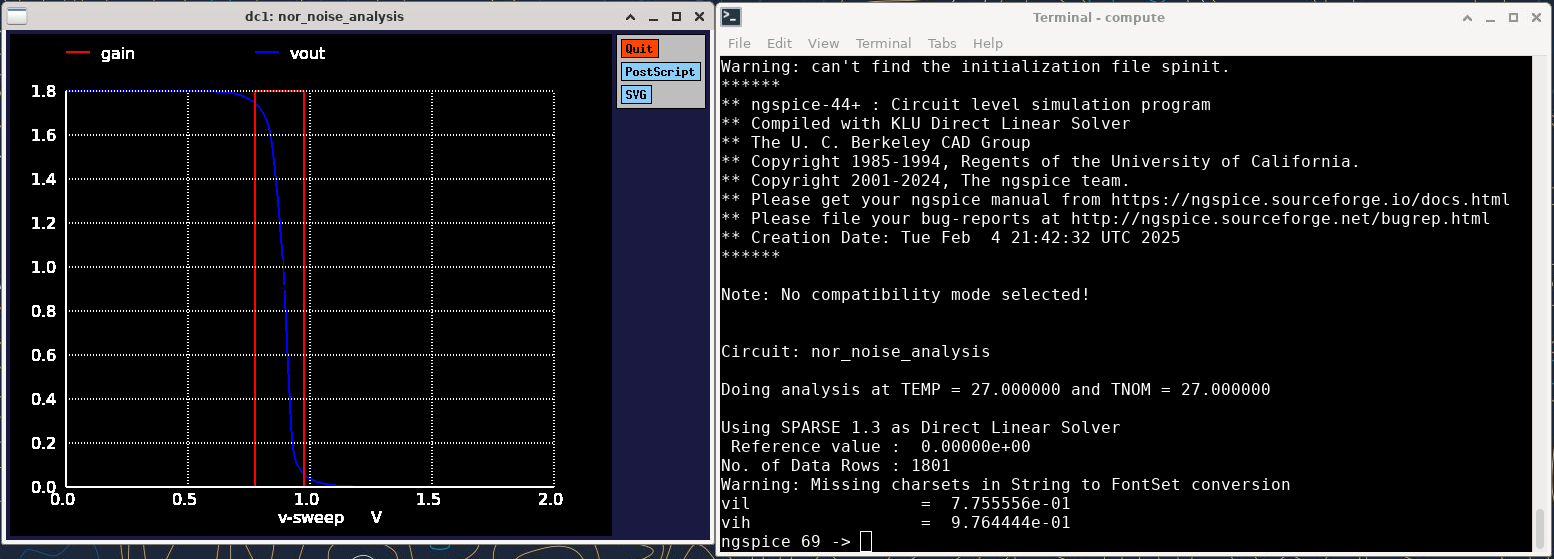
\includegraphics[width=0.8\textwidth]{nor_noise_analysis.png}}
		\caption{Noise Analysis Results from Netlist Simulation}
		\label{fig::nor_noise_analysis}
	\end{figure}
	
	\begin{figure}[H]
		\centerline{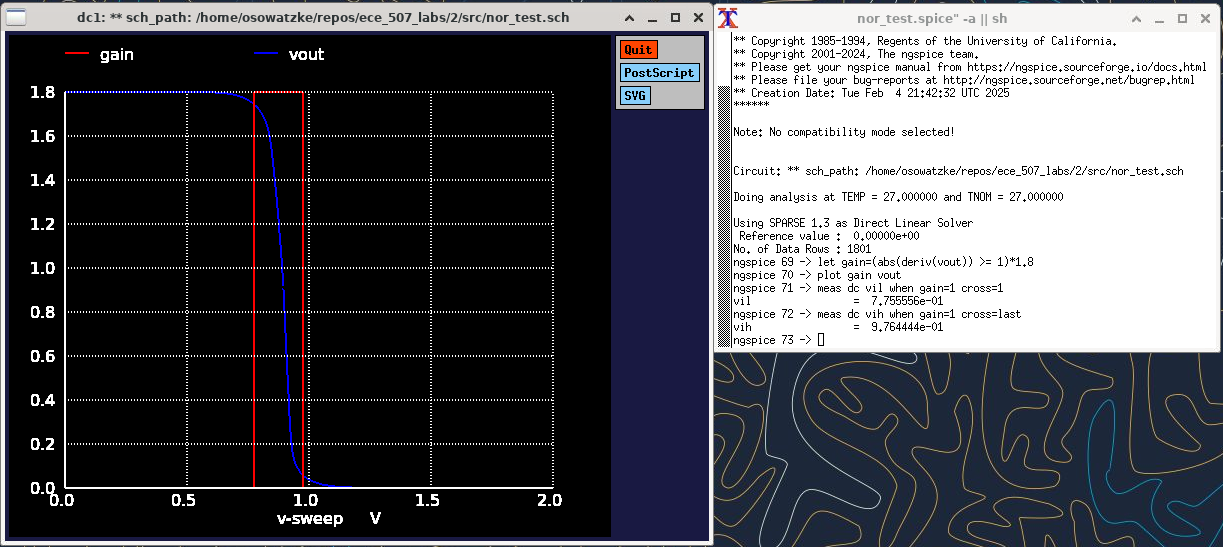
\includegraphics[width=0.8\textwidth]{nor_noise_analysis_schem.png}}
		\caption{Noise Analysis Results from Schematic Simulation}
		\label{fig::nor_noise_analysis_schem}
	\end{figure}
	
	\begin{table}[H]
	\begin{center}
	\caption{Noise Margins from Netlist Simulation}
	\label{table::nor_gate_noise_analysis}
	\begin{tabular}{| c | c | c | c | c | c |}
		\hline
		\texttt{a} & \texttt{b} & \texttt{Vih} & \texttt{Vil} & \texttt{Nmh} & \texttt{Nml} \\
		\hline	
		$0 \rightarrow 1$ & $0$ & $0.9764 \text{V}$ & $0.7756 \text{V}$ & $0.8326 \text{V}$ & $0.7756 \text{V}$\\
		\hline	
		$0$ & $0 \rightarrow 1$ & $1.0134 \text{V}$ & $0.7706 \text{V}$ & $0.7660 \text{V}$ & $0.7706 \text{V}$\\
		\hline	
		$0 \rightarrow 1$ & $0 \rightarrow 1$ & $0.7006 \text{V}$ & $0.8844 \text{V}$ & $0.9156 \text{V}$ & $0.7006 \text{V}$\\
		\hline
	\end{tabular}
	\end{center}
	\end{table}
	
	\begin{table}[H]
	\begin{center}
	\caption{Noise Margins from Schematic Simulation}
	\label{table::nor_gate_noise_analysis_schem}
	\begin{tabular}{| c | c | c | c | c | c |}
		\hline
		\texttt{a} & \texttt{b} & \texttt{Vih} & \texttt{Vil} & \texttt{Nmh} & \texttt{Nml} \\
		\hline	
		$0 \rightarrow 1$ & $0$ & $0.9764 \text{V}$ & $0.7756 \text{V}$ & $0.8326 \text{V}$ & $0.7756 \text{V}$\\
		\hline	
		$0$ & $0 \rightarrow 1$ & $1.0134 \text{V}$ & $0.7706 \text{V}$ & $0.7660 \text{V}$ & $0.7706 \text{V}$\\
		\hline	
		$0 \rightarrow 1$ & $0 \rightarrow 1$ & $0.7006 \text{V}$ & $0.8844 \text{V}$ & $0.9156 \text{V}$ & $0.7006 \text{V}$\\
		\hline
	\end{tabular}
	\end{center}
	\end{table}
	
	\subsubsection{Delay Analysis}
	\begin{figure}[H]
		\lstinputlisting[style=nocoloring,frame=single,basicstyle=\fontsize{7}{7}\selectfont\ttfamily]{./src/nor_delay_analysis.spice}
		\caption{SPICE Test Circuit to Perform Delay Analysis on Netlist}
		\label{fig::nor_delay_analysis_test_circuit}
	\end{figure}
	
	\begin{figure}[H]
		\centerline{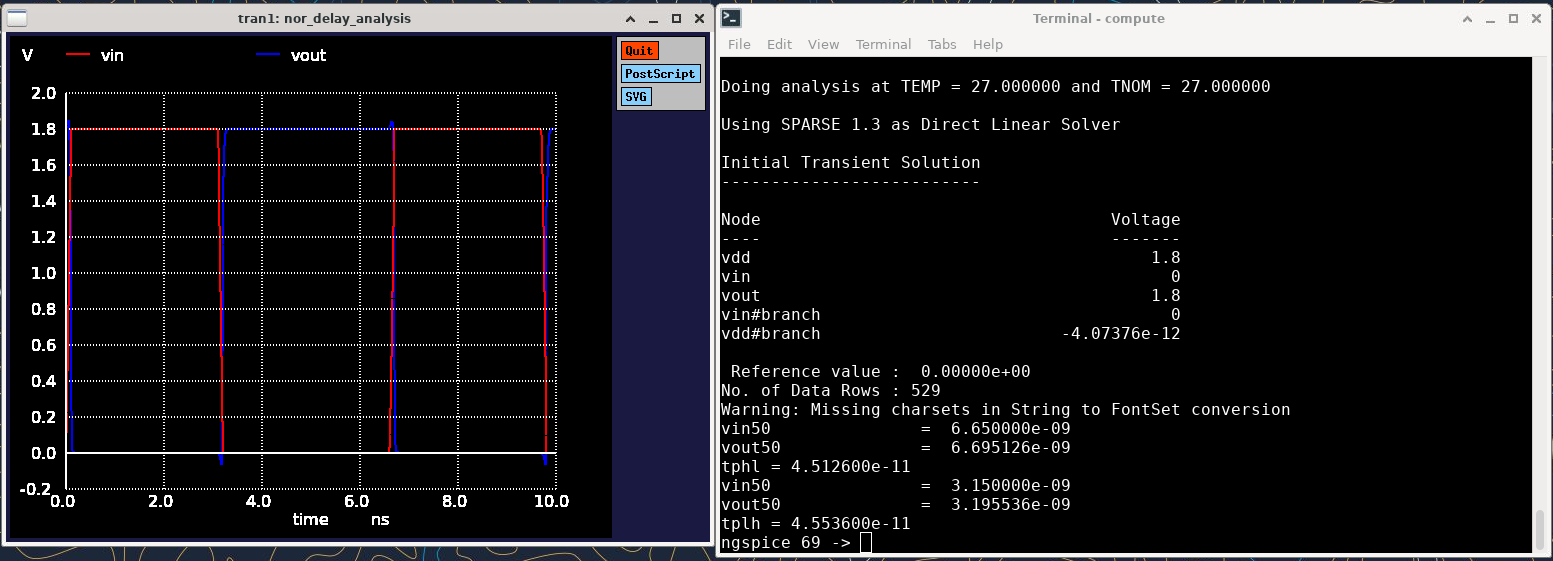
\includegraphics[width=0.8\textwidth]{nor_delay_analysis.png}}
		\caption{Delay Analysis Results from Netlist Simulation}
		\label{fig::nor_delay_analysis}
	\end{figure}
	
	\begin{figure}[H]
		\centerline{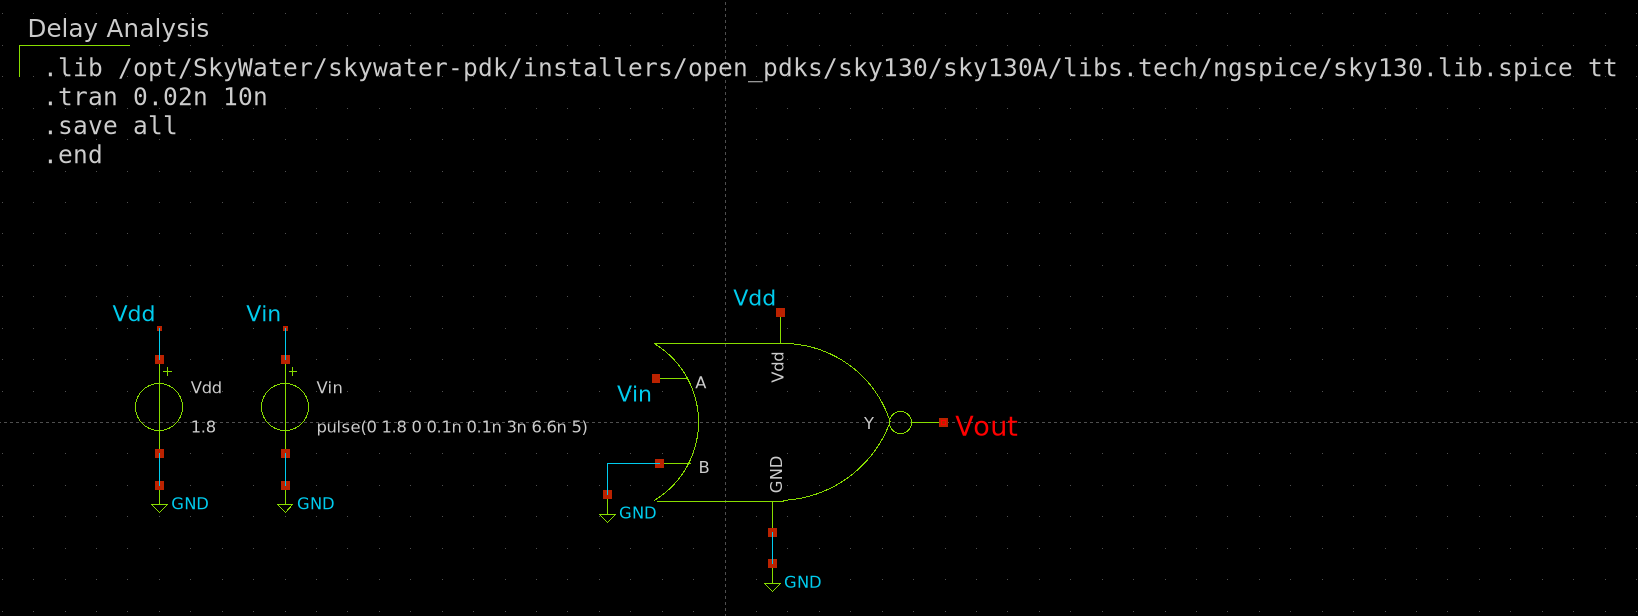
\includegraphics[width=0.8\textwidth]{nor_delay_analysis_test_circuit.png}}
		\caption{Schematic Test Circuit for NOR Gate Delay Analysis}
		\label{fig::nor_delay_analysis_test_circuit_schem}
	\end{figure}
	
	\begin{figure}[H]
		\centerline{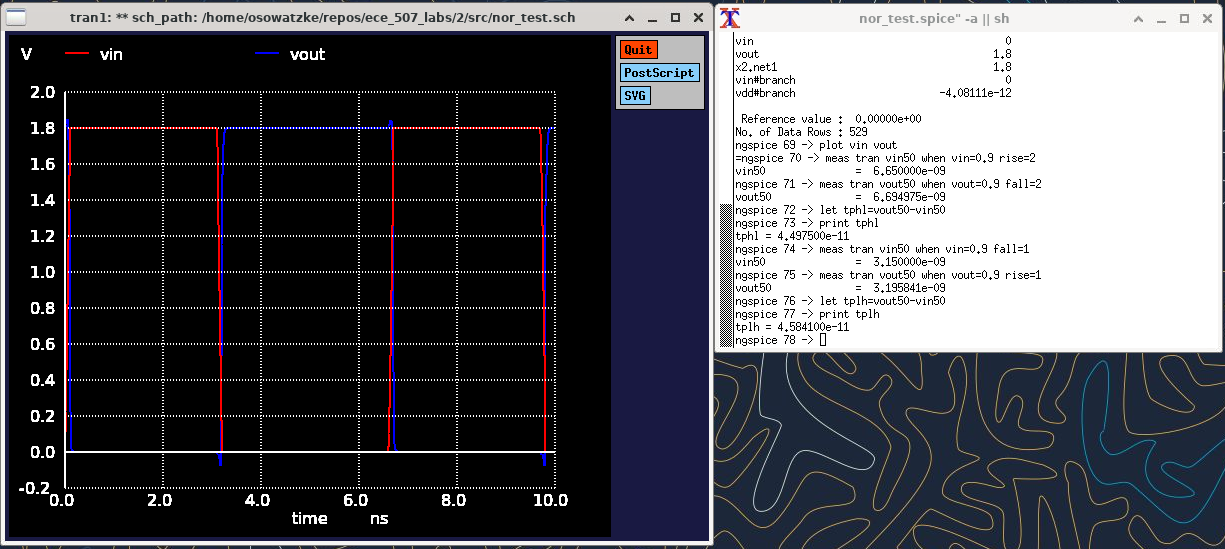
\includegraphics[width=0.8\textwidth]{nor_delay_analysis_schem.png}}
		\caption{Delay Analysis Result from Schematic Simulation}
		\label{fig::nor_delay_analysis_schem}
	\end{figure}
	
	\begin{table}[H]
	\begin{center}
	\caption{Delay from Netlist Simulation}
	\label{table::nor_gate_delay_analysis}
	\begin{tabular}{| c | c | c || c | c | c |}
		\hline
		\texttt{a} & \texttt{b} & \texttt{tphl} & \texttt{a} & \texttt{b} & \texttt{tplh} \\
		\hline	
		$0 \rightarrow 1$ & $0$ & $45.126\ \text{ps}$ & $1 \rightarrow 0$ & $0$ & $45.536\ \text{ps}$\\
		\hline	
		$0$ & $0 \rightarrow 1$ & $30.061\ \text{ps}$ & $0$ & $1 \rightarrow 0$ & $30.975\ \text{ps}$\\
		\hline	
		$0 \rightarrow 1$ & $0 \rightarrow 1$ & $24.033\ \text{ps}$ & $1 \rightarrow 0$ & $1 \rightarrow 0$ & $43.556\ \text{ps}$\\
		\hline
	\end{tabular}
	\end{center}
	\end{table}
	
	\begin{table}[H]
	\begin{center}
	\caption{Delay from Schematic Simulation}
	\label{table::nor_gate_delay_analysis_schem}
	\begin{tabular}{| c | c | c || c | c | c |}
		\hline
		\texttt{a} & \texttt{b} & \texttt{tphl} & \texttt{a} & \texttt{b} & \texttt{tplh} \\
		\hline	
		$0 \rightarrow 1$ & $0$ & $44.975\ \text{ps}$ & $1 \rightarrow 0$ & $0$ & $45.841\ \text{ps}$\\
		\hline	
		$0$ & $0 \rightarrow 1$ & $29.139\ \text{ps}$ & $0$ & $1 \rightarrow 0$ & $29.942\ \text{ps}$\\
		\hline	
		$0 \rightarrow 1$ & $0 \rightarrow 1$ & $22.437\ \text{ps}$ & $1 \rightarrow 0$ & $1 \rightarrow 0$ & $40.998\ \text{ps}$\\
		\hline
	\end{tabular}
	\end{center}
	\end{table}
	
	\subsubsection{Power Analysis}
	\begin{figure}[H]
		\lstinputlisting[style=nocoloring,frame=single,basicstyle=\fontsize{7}{7}\selectfont\ttfamily]{./src/nor_power_analysis.spice}
		\caption{SPICE Test Circuit to Perform Power Analysis on Netlist}
		\label{fig::nor_power_analysis_test_circuit}
	\end{figure}
	
	\begin{figure}[H]
		\centerline{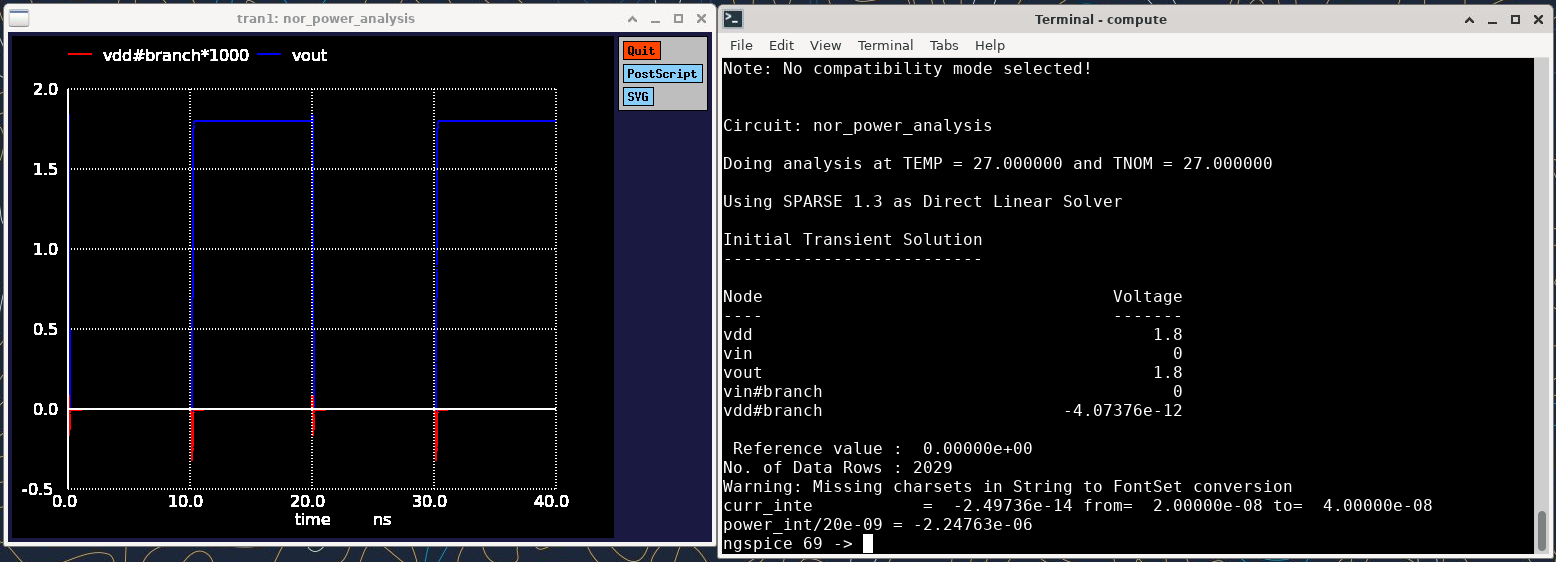
\includegraphics[width=0.8\textwidth]{nor_power_analysis.png}}
		\caption{Power Analysis Results from Netlist Simulation}
		\label{fig::nor_power_analysis}
	\end{figure}
	
	\begin{figure}[H]
		\centerline{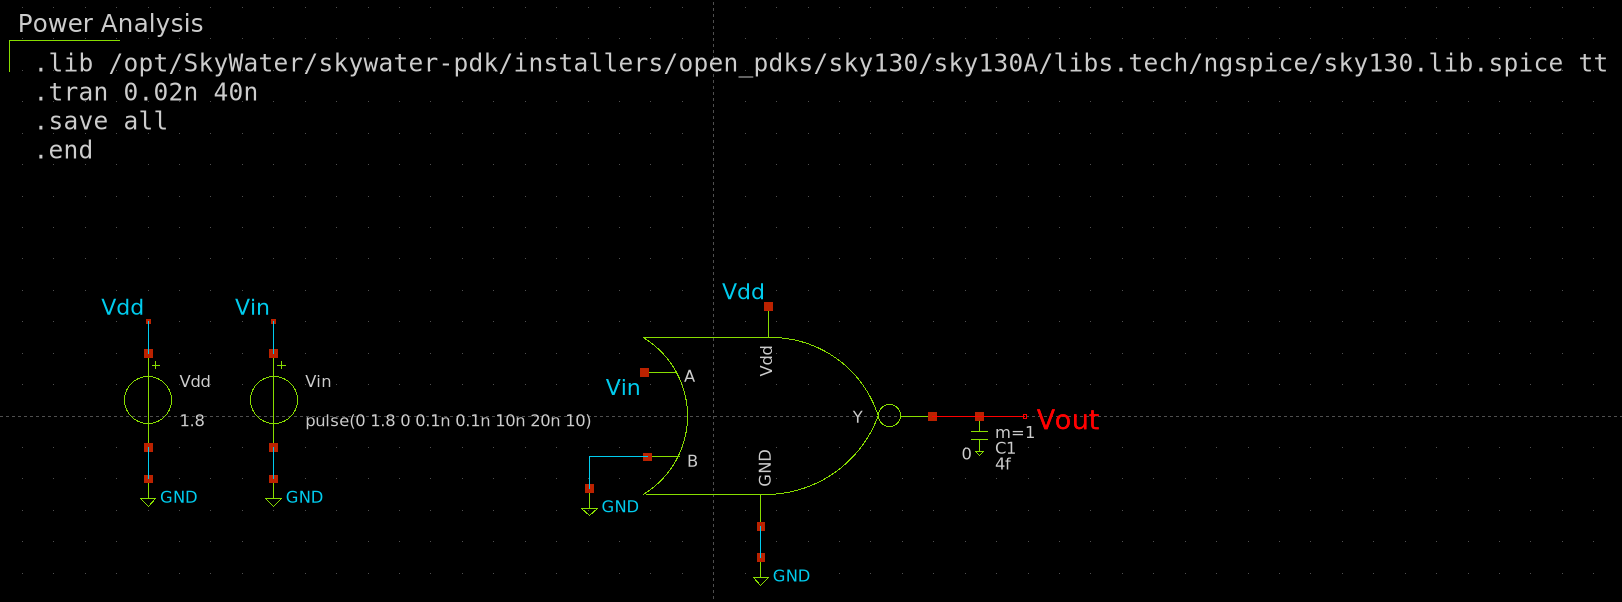
\includegraphics[width=0.8\textwidth]{nor_power_analysis_test_circuit.png}}
		\caption{Schematic Test Circuit for NOR Gate Power Analysis}
		\label{fig::nor_power_analysis_test_circuit_schem}
	\end{figure}
	
	\begin{figure}[H]
		\centerline{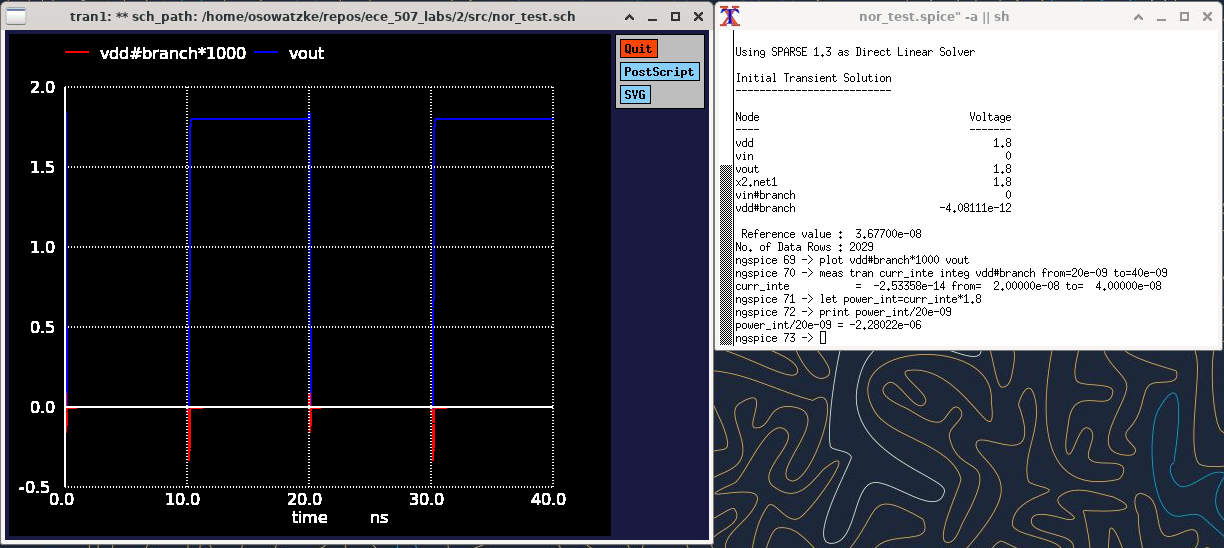
\includegraphics[width=0.8\textwidth]{nor_power_analysis_schem.png}}
		\caption{Power Analysis Results from Schematic Simulation}
		\label{fig::nor_power_analysis_schem}
	\end{figure}
	
	\begin{table}[H]
	\begin{center}
	\caption{Power Consumption from Netlist Simulation}
	\label{table::nor_gate_power_analysis}
	\begin{tabular}{| c | c | c |}
		\hline
		\texttt{a} & \texttt{b} & \texttt{Power}\\
		\hline	
		$0 \rightarrow 1 \rightarrow 0$ & $0$ & $2.24763{\mu}W$ \\
		\hline	
		$0$ & $0 \rightarrow 1 \rightarrow 0$ & $1.43645{\mu}W$ \\
		\hline	
		$0 \rightarrow 1 \rightarrow 0$ & $0 \rightarrow 1 \rightarrow 0$ & $1.67940{\mu}W$\\
		\hline
	\end{tabular}
	\end{center}
	\end{table}
	
	\begin{table}[H]
	\begin{center}
	\caption{Power Consumption from Schematic Simulation}
	\label{table::nor_gate_power_analysis_schem}
	\begin{tabular}{| c | c | c |}
		\hline
		\texttt{a} & \texttt{b} & \texttt{Power}\\
		\hline	
		$0 \rightarrow 1 \rightarrow 0$ & $0$ & $2.28022{\mu}W$ \\
		\hline	
		$0$ & $0 \rightarrow 1 \rightarrow 0$ & $1.37674{\mu}W$ \\
		\hline	
		$0 \rightarrow 1 \rightarrow 0$ & $0 \rightarrow 1 \rightarrow 0$ & $1.61932{\mu}W$\\
		\hline
	\end{tabular}
	\end{center}
	\end{table}
	
	\bibliographystyle{IEEEtran}
	\bibliography{IEEEabrv,sources}
\end{document}